%% ----------------------------------------------------------------
%% Thesis.tex -- MAIN FILE (the one that you compile with LaTeX)
%% ---------------------------------------------------------------- 

% Set up the document
\documentclass[a4paper, 11pt, oneside]{Thesis}  % Use the "Thesis" style, based on the ECS Thesis style by Steve Gunn
\graphicspath{Figures/}  % Location of the graphics files (set up for graphics to be in PDF format)

% Include any extra LaTeX packages required
\usepackage[square, numbers, comma, sort&compress]{natbib}  % Use the "Natbib" style for the references in the Bibliography
\usepackage{verbatim}  % Needed for the "comment" environment to make LaTeX comments
\usepackage{vector}  % Allows "\bvec{}" and "\buvec{}" for "blackboard" style bold vectors in maths
\hypersetup{urlcolor=blue, colorlinks=true}  % Colours hyperlinks in blue, but this can be distracting if there are many links.
\usepackage{amsfonts}
\usepackage{amsmath}

%% ----------------------------------------------------------------
\begin{document}
\frontmatter      % Begin Roman style (i, ii, iii, iv...) page numbering

% Set up the Title Page
\title  {Medical Image Analysis of in-vivo hearts}
\authors  {\texorpdfstring
            {\href{http://www.cim.mcgill.ca/students/Goblot.Damien.html}{Damien Goblot}}
            {Damien Goblot}
            }
\addresses  {\groupname\\\deptname\\\univname}  % Do not change this here, instead these must be set in the "Thesis.cls" file, please look through it instead
\date       {\today}
\subject    {}
\keywords   {}

\maketitle
%% ----------------------------------------------------------------

\setstretch{1.3}  % It is better to have smaller font and larger line spacing than the other way round

% Define the page headers using the FancyHdr package and set up for one-sided printing
\fancyhead{}  % Clears all page headers and footers
\rhead{\thepage}  % Sets the right side header to show the page number
\lhead{}  % Clears the left side page header

\pagestyle{fancy}  % Finally, use the "fancy" page style to implement the FancyHdr headers

%% ----------------------------------------------------------------
% Declaration Page required for the Thesis, your institution may give you a different text to place here
\Declaration{

\addtocontents{toc}{\vspace{1em}}  % Add a gap in the Contents, for aesthetics

I, AUTHOR NAME, declare that this thesis titled, `THESIS TITLE' and the work presented in it are my own. I confirm that:

\begin{itemize} 
\item[\tiny{$\blacksquare$}] This work was done wholly or mainly while in candidature for a research degree at this University.
 
\item[\tiny{$\blacksquare$}] Where any part of this thesis has previously been submitted for a degree or any other qualification at this University or any other institution, this has been clearly stated.
 
\item[\tiny{$\blacksquare$}] Where I have consulted the published work of others, this is always clearly attributed.
 
\item[\tiny{$\blacksquare$}] Where I have quoted from the work of others, the source is always given. With the exception of such quotations, this thesis is entirely my own work.
 
\item[\tiny{$\blacksquare$}] I have acknowledged all main sources of help.
 
\item[\tiny{$\blacksquare$}] Where the thesis is based on work done by myself jointly with others, I have made clear exactly what was done by others and what I have contributed myself.
\\
\end{itemize}
 
 
Signed:\\
\rule[1em]{25em}{0.5pt}  % This prints a line for the signature
 
Date:\\
\rule[1em]{25em}{0.5pt}  % This prints a line to write the date
}
\clearpage  % Declaration ended, now start a new page

%% ----------------------------------------------------------------
% The "Funny Quote Page"
\pagestyle{empty}  % No headers or footers for the following pages

\null\vfill
% Now comes the "Funny Quote", written in italics
\textit{``Write a funny quote here.''}

\begin{flushright}
If the quote is taken from someone, their name goes here
\end{flushright}

\vfill\vfill\vfill\vfill\vfill\vfill\null
\clearpage  % Funny Quote page ended, start a new page
%% ----------------------------------------------------------------

% The Abstract Page
\addtotoc{Abstract}  % Add the "Abstract" page entry to the Contents
\abstract{
\addtocontents{toc}{\vspace{1em}}  % Add a gap in the Contents, for aesthetics

The Thesis Abstract is written here (and usually kept to just this page). The page is kept centered vertically so can expand into the blank space above the title too\ldots

}

\clearpage  % Abstract ended, start a new page
%% ----------------------------------------------------------------

\setstretch{1.3}  % Reset the line-spacing to 1.3 for body text (if it has changed)

% The Acknowledgements page, for thanking everyone
\acknowledgements{
\addtocontents{toc}{\vspace{1em}}  % Add a gap in the Contents, for aesthetics

The acknowledgements and the people to thank go here, don't forget to include your project advisor\ldots

}
\clearpage  % End of the Acknowledgements
%% ----------------------------------------------------------------

\pagestyle{fancy}  %The page style headers have been "empty" all this time, now use the "fancy" headers as defined before to bring them back


%% ----------------------------------------------------------------
\lhead{\emph{Contents}}  % Set the left side page header to "Contents"
\tableofcontents  % Write out the Table of Contents

%% ----------------------------------------------------------------
\lhead{\emph{List of Figures}}  % Set the left side page header to "List if Figures"
\listoffigures  % Write out the List of Figures

%% ----------------------------------------------------------------
\lhead{\emph{List of Tables}}  % Set the left side page header to "List of Tables"
\listoftables  % Write out the List of Tables

%% ----------------------------------------------------------------
\setstretch{1.5}  % Set the line spacing to 1.5, this makes the following tables easier to read
\clearpage  % Start a new page
\lhead{\emph{Abbreviations}}  % Set the left side page header to "Abbreviations"
\listofsymbols{ll}  % Include a list of Abbreviations (a table of two columns)
{
% \textbf{Acronym} & \textbf{W}hat (it) \textbf{S}tands \textbf{F}or \\
\textbf{LAH} & \textbf{L}ist \textbf{A}bbreviations \textbf{H}ere \\

}

%% ----------------------------------------------------------------
\clearpage  % Start a new page
\lhead{\emph{Physical Constants}}  % Set the left side page header to "Physical Constants"
\listofconstants{lrcl}  % Include a list of Physical Constants (a four column table)
{
% Constant Name & Symbol & = & Constant Value (with units) \\
Speed of Light & $c$ & $=$ & $2.997\ 924\ 58\times10^{8}\ \mbox{ms}^{-\mbox{s}}$ (exact)\\

}

%% ----------------------------------------------------------------
\clearpage  %Start a new page
\lhead{\emph{Symbols}}  % Set the left side page header to "Symbols"
\listofnomenclature{lll}  % Include a list of Symbols (a three column table)
{
% symbol & name & unit \\
$a$ & distance & m \\
$P$ & power & W (Js$^{-1}$) \\
& & \\ % Gap to separate the Roman symbols from the Greek
$\omega$ & angular frequency & rads$^{-1}$ \\
}
%% ----------------------------------------------------------------
% End of the pre-able, contents and lists of things
% Begin the Dedication page

\setstretch{1.3}  % Return the line spacing back to 1.3

\pagestyle{empty}  % Page style needs to be empty for this page
\dedicatory{For/Dedicated to/To my\ldots}

\addtocontents{toc}{\vspace{2em}}  % Add a gap in the Contents, for aesthetics


%% ----------------------------------------------------------------
\mainmatter	  % Begin normal, numeric (1,2,3...) page numbering
\pagestyle{fancy}  % Return the page headers back to the "fancy" style

% Include the chapters of the thesis, as separate files
% Just uncomment the lines as you write the chapters

\chapter{Literature Review}

\section{Zurich + Oxford confidential proposal}

\subsection{Definition}

DTI definitions:
• ADC (apparent diffusion coefficient), measured in $mm^2/s$: it is a measure of how quickly the water molecules spread out
due to diffusion, defined as the mean of the diagonal of the diffusion tensor. Consider the drawing A, where the red line shows the typical diffusion of a water molecule, randomly moving around – the black ball shows this molecules diffusion speed and direction. In constricted regions (e.g. inside cells) water is constrained, and the mean diffusion (apparent diffusion coefficient, or ADC) is low, while in regions where the motion of the water molecules is unconstrained, ADC is high . For example, in the drawing below (adapted from http://www.cabiatl.com/CABI/resources/dti-analysis/), water is diffusing faster in A than B.
• FA (fractional anisotropy), unitless: it is a measure of how much the diffusion is restricted in different directions; an FA of 0 means that diffusion is wholly isotropic (equal in all directions), while an FA of 1 means that diffusion is solely along one direction. This is defined as the standard deviation of the eigenvalues of the diffusion tensors divided by the root mean square of the eigenvalues. For example, in drawing C the water is moving isotropically, while
in D the water is moving anisotropically.
• HA (helix angle), measured in degrees: it shows the direction along which water molecules preferentially diffuse, This has been shown by histology to agree with the orientation of the myofibres. It is defined as the angle the principal eigenvector of the diffusion tensor makes with the vector pointing circumferentially around the short axis of the myocardium.


\subsection{Article}

The paper aims at establishing cardiovascular magnetic resonance (CMR) imaging techniques to efficiently evaluate myocardial irreversible injury, especially for patients presenting acute myocardial infection (MI).
Specifically, the goal is to assess the lack of integrity and the subsequent rearrangement of the myocardial bundles, to be able to use these to predict arrhythmias and establish new predictors of LV remodeling (?).\\
The group has shown that L2W and LGE CMR are not suitable methods for assessment of irreversible injury acutely. Instead, they plan on using, based on DTI, apparent diffusion coefficient (ADC) and fractional anisotropy (FA) and by their quantification of myocardial fiber integrity imaging have a tool to assess irreversibility of myocardial injury.\\

A recently developed time-resolved CMR 4D flow imaging technique for quantification of blood flow in the whole heart throughout the cardiac
cycle enables assessment of the kinetic energy (KE) changes of the individual LV flow components.

Quantifying the degree of KE loss of the flow over time and relating this to the underlying myocardial fiber arrangement would allow us to establish a novel potential predictor of LV dilation and heart failure, beyond
the conventional EF-based clinical stratification currently used.\\

The primary endpoints and readouts of this proposal are: (1) the degree of disruption and re-arrangement of myocardial fibre bundles (characterized by ADC/FA maps and HA distribution) as predictors of irreversible injury, defined by LGE scarred myocardium and lack of functional recovery at 6 months; (2) the degree of acute myocardial bundle re-arrangement (defined as HA distribution) in the peri-infarct zone (defined on 6 months LGE) as a predictor of ventricular arrhythmias assessed acutely, 4 weeks and 6 months on a 24h Holter monitoring system, respectively; (3) The KE loss of intraventricular blood flow (assessed by 4D flow) in the early phases post MI as predictor of adverse LV remodeling at 18 months (assessed by increase in end-systolic volume and decrease in EF between day 1 and 18 months). Dedicated post-processing tools will be developed by the post-doctoral research scientist, who will also
support the data analysis.

\section{PNAS-2012-Savadjiev-9248-53}

This article aims at explaining how myofibers are bundled in the heart wall while economizing fiber length and optimizing ventricular ejection volume as they contract. This arrangement is of a minimal surface, the generalized helicoid.\\
They use mathematical models involving the angular change in the appropriate local coordinate frame. Their model is based on the Maurer Cartan's moving frame construction, where the local coordinate frame is more meaningful in a small than in a too large frame where the tangent plane approximation becomes less accurate.\\
They show that fibers are packed together to achieve the helicoidal organization, and that this minimal surface structure can be maintained during the beat cycle. The improvement since previous research is to describe volumetric bundles of fibers instead of solely an individual description of them, and the analysis of the fiber orientation in 3D. They also consider the apex in their study, which was so far excluded from former analysis.\\
The helicoid is obtained if you go through the heart wall, in any direction from the epicardium to the endocardium. The histograms indeed show a homogeneous value for $K_B$, and different $\neq 0$ ($2.63° \leq \mu \geq 7.63°$), whereas values for $K_T$ and $K_N$ are centered around 0. $K_B$ has the effect of creating rotated copies of the same fibers in the z direction, therefore in planes parallel to the x-y plane.

\section{Strijkers et al-2009-NMR in Biomedicine}

\subsection{Definitions}

remodeling: change in size, shape and function of the heart

\subsection{Article}

They use in this study left ventricular remodeling in a mouse using DTI. They induce a myocardial infarction by permanent ligation of the left anterior descending coronary artery. Then they perform ex-vivo DTI measurements 7,14,28 and 60 days after ligation.\\
After myocardial infarction, the mouse hearts show an important wall thinning in the infarcted area, a heart mass increase of up to 70\%.
The infarct at 7 days consisted of unstructured tissue with residual necrosis and infiltration of macrophages and myofibroblasts. At 14 days after infarction, the necrotic tissue had disappeared and collagen fibers were starting to appear. From 28 to 60 days, the infarct had fully developed into a mature scar.\\
The infarcted heart wall was too thin to have relevant data of the change in helix angles, but the ADC increased with infarction, as well as the FA that was maximal at 28 days. The DA is significantly greater in the infarcted areas as well.\\
After myocardial infarction, cardiomyocytes are replaced by scar tissue, which lacks contractile properties. This tissue expands and becomes thinner.

\section{Brain choline concentration \~{}}

They found that choline concentration measured by 1H MRS in DTI normal-appearing tissue located around the ischemic lesion within the first 26 hours from stroke onset was elevated in those voxels that became infarcted on DTI within the next few days. Moreover, the degree of ischemic expansion was associated with the degree of elevation of choline concentration. Further studies are required to determine whether choline concentration is a reliable, sensitive, or specific measure for predicting infarct growth, including identification of the potential threshold values, and therefore could be used to support treatment decisions in routine practice.

\section{Diffusion tensor magnetic resonance imaging}

\subsection{Definitions}

LHF and RHF: left and right-handed helical fiber

\subsection{Article}

This paper focuses on the use of DT-MRI to show how they can help as indicators of fiber architecture remodeling after an infarct on human data.\\
They show that trace ADC is significantly increased in the infarct zone, which is consistent with the findings on rat heart data. This increase is caused by the presence of scar tissue and therefore increase in the extracellular space, thus less restriction for diffusion.
FA in the infarct zone significantly decreases in the infarct zone, once again in line with the results obtained from rat data. They also find that 26 days after acute MI, trace ADC and FA in each viability zone showed significant inverse correlation.\\
The helix angle distribution of the myocardial fibers was significantly altered across the 3 zones.\\
RHF\% decreased and LHF\% increased in the infarct zone, and the opposite occured in the remote zone.\\
Hypothesis brought by this paper: area most susceptible to ischemia is the subendocardial area. Therefore, RHF had the most severe loss in the infarct zone. Second, an increase in LHF\% in the infarct zone may represent a remodeling process triggered to compensate for the loss of RHF in the infarct zone and to keep the balanced ratio of $\frac{\text{LHF\%} \times \text{RHF\%}}{\text{CF\%}}$. Third, the RHF\% increase in remote compensatory hypertrophy may be an adaptive remodeling response to the increase in wall stress.

\section{Serial diffusion tensor mri and tractography of the mouse heart in-vivo \~{}}

Measurements of RV long axis displacement by CMR tagging showed more significant differences between the groups studied than did RV-EF. It was reproducible, quick and easy to apply and analyse. They insist on the insensitivity of the RV-EF as a marker of change in the RV myocardial contractile function.

\section{Myocardial diffusion tensor imaging using diffusion-prepared ssfp \~{} Treatment?}

In TM patients prospectively observed for 18 months, at the dosages used in the real world, combined DFP+DFO regimen and DFP in monotherapy were not significantly different in removing myocardial iron and improving heart function, while combined DFP+DFO therapy was more effective in the hepatic iron clearance. Combined DFP+DFO regimen confirmed its higher efficacy versus subcutaneous DFO in removing heart and liver iron, without an additional effect on the heart function. Further randomized controlled trials at fixed therapeutic schedules should be designed to verify these findings.

\section{Cardiovascular magnetic resonance characterization of peri-infarct zone remodeling following myocardial infarction}

The risk of sudden death is the highest in the 30 days following an MI. Islands of viable myocardium, surrounded by regions of myocardial scar, can produce the substrate for monomorphic ventricular tachycardia (VT), which is a significan risk factor for sudden cardiac death.
The 2 major findings of this study are: a temporal change in peri infarct zone (PIZ) size detected with LGE-CMR, and myocardial strain patterns change during the post-MI remodeling process.
Cardiac wound repair, after MI, involves temporarily overlapping phases which include an inflammatory phase and tissue remodeling phase.
Even with unperfectly reliable evaluation of the PIZ, the size and mass of it decreases after MI, before it stabilizes.

\section{Reese et al-1995-Magnetic Resonance in Medicine}

\section{Maurer-Cartan Forms for Fields on Surfaces: Application to Heart Fiber Geometry}

Based on Maurer-Cartan form and methods applied from this basis, the goal of the paper is to apply it to moving frames in a rigorous way, the generation of various geometrical embeddings - the heart in particular. The Maurer-Cartan form is an operator that measures the differential structure of a manifold, and it is applied to study the geometrical characteristics  of the manifold under consideration. In this article they apply the theory of moving frames in the reverse direction so that the Maurer-Cartan forms are used to generate manifolds or embeddings based on assumptions of their differential structure --> this is what we will use in our research.\\
This idea can be used to characterize a smooth frame field in the three dimensions as a parametrization on the space of the Maurer-Cartan connection forms.\\
They also develop and compare a number of fitting method that will be very helpful in fitting our data.\\
Let's define the local frame field $\mathbf{F = [f_1 , f_2 , f_2]^T} : \mathbb{R}^3 \to \mathbb{R}^3$.\\
We have by construction: $\mathbf{F = A[e_1 , e_2 , e_3]^T = AE}$.\\
Therefore we get: $d \mathbf{f_i} = \sum_j c_{i,j}\mathbf{f_j}$.\\
The Maurer-Cartan matrix is skew symmetric: $\mathbf{C} = \begin{bmatrix}0 & c_{1,2} & c_{1,3} \\ -c_{1,2} & 0 & c_{2,3} \\ -c_{1,3} & -c_{2,3} & 0
\end{bmatrix}$.\\
Using these notations we can define $c_{i,j,k}$ to be the coefficient of the turning of $\mathbf{f_i}$ towards $\mathbf{f_j}$ when we move (our position) towards $\mathbf{f_k}$.\\

\section{Test}

Citing (copy pasting the parts 3. and 3.2 of Emmanuel's Pami paper)...

We want to fit the model by computing the connection forms $c_{ijk}$ for every location (voxel) of the data we are looking at. In order to do so, we minimize the energy term described in the part 3.2 \cite{pami2015}. We solve the optimization problem using the standard Nelder-Mead algorithm that we implemented for our needs.
As described in part 5.2 of 
Our estimate of the frame field orientation is computed thanks to our connection forms, and this is also thanks to our connection forms that we are able to run tractography that we can see in Figure 1. Suppose I start from a given voxel, when I move towards a direction I use the connection form parameters that give me the change of orientation when I move in that direction and that helps me trace the actual fiber orientation, following its inner connection form parameters. Our tractography in that sense is not just connecting points between fibers but really locally estimating the parameters for a given fiber and tracing only from this starting point informations.
Our error of fit therefore explains very clearly if the parameters for a given fiber are accurate enough to describe the orientation of its neighbors.


\chapter{Introduction}

The technological improvement of noninvasive medical imaging techniques in the past couple of decades has allowed us to get a better understanding of the heart's structure \cite{sinusas2008multimodality}. This is also thanks to the increasing amount of data that can be collected more and more easily and with better definition as time goes by. \\
As the imaging techniques get better \cite{shaw2010cardiovascular}, the analysis of the images we get still plays a major role in understanding the causes and effects of the disease and has to be used in a clever way to drive further down the number of cardiovascular diseases that is still the leading global cause of death \cite{mozaffarian2015heart} since 1900 (except for the year 1918). \\
Although
1
2
new developments in imaging modalities can sometimes be revolutionary – such as in
vivo diffusion imaging [119] which can be used to construct a three-dimensional map
of muscle fibers in the beating heart – these will only add to the mountain of cardiac
measurements that are already available. One of the main challenges of cardiovascular
imaging is to be able to efficiently process and provide visualizations of dense
and complex cardiac data in a way that is useful for the clinician, thereby warranting
the need for powerful and intuitive computational imaging tools. The analysis
of cardiac muscle fibers is of particular interest since these play a key role in the
mechanical function, electrophysiology and remodeling processes of the heart [40].
Various pathologies disrupt the organization of these fibers which can impair the
ability of the heart muscle to operate efficiently [9]. Modern treatments of conditions
involving a disorganization of heart fibers include tissue engineering methods,
in which a synthetic material or stem cell therapy are used to restore cardiac contractile
muscle properties in vitro [17, 50, 51, 118, 137], and mechanical ventricular
restoration techniques that involve reconstruction, cauterization, and/or ablation of
impaired or necrotic regions [6, 25, 45, 105]. Computational models of heart fibers
could potentially be used to assist and augment these procedures via statistical and
geometrical priors.
Early histological work has shown that cardiac fibers wrap around the ventricles
in a highly smooth and regular manner [123]. Other local characterizations have long
been established, such as the helix angle, which is a measure of fiber orientation with
respect to the heart wall and is a commonly – and often solely – used descriptor of
local fiber geometry [32]. Other local models of cardiac fibers such as ruled-based
3
models [8] and atlas-based models [61] can be useful in generating and comparing
healthy anatomy, but they lack in intuition and adaptability for characterizing the
more complex geometry that arises in pathological tissue. Various anatomical models
have also been proposed to explain the global organization of cardiac fibers, based on
both empirical and mathematical considerations [34,86], but these provide high-level
generalizations that do not necessarily translate well to the analysis of real cardiac
tissue.
1.1 Objectives of this Thesis
Whereas existing models of heart fiber organization can be useful from an educational
perspective, they lack the necessary precision for quantifying the local
geometry of fibers in real anatomy. The main objective of this thesis is the development
of novel computational techniques for the analysis of three-dimensional frame
fields, with an application to the modeling of cardiac fibers. Our goals are for these
tools to be intuitive, to have a solid theoretical underpinning, to extend prior models
in the literature and to lead to algorithms that can be readily applied to cardiac
diffusion magnetic resonance imaging data.

In this thesis we start from our knowledge of Maurer-Cartan connection form description of the fibers of the heart \cite{7053934}. From this basis we try and analyze the possible impacts that an infarcted heart can have on the fiber orientation in the infarct area and areas away from the infarcted regions.

\chapter{} % Introduction

\chapter{Literature Review}

\section{Cardiac Diffusion MRI}

Magnetic Resonance Imaging (MRI) is the imaging method that was used to acquire the data on which are results are based. It is non-invasive and especially adapted to soft-tissues. We will explain briefly how it works and what information it gives us.

\subsection{Physics of MRI}

Magnetic Resonance acquisitions rely on the physical properties of the body, and more specifically the most abundant nucleus which is hydrogen (H). Indeed water molecules represent more than 70\% of the entire body composition. This hydrogen nucleus consists of 1 proton and 1 electron of opposite electrical charge. The relative position of the electron in respect to the proton leads to different electron spin that is a property of this atom and makes it behave like a magnetic dipole. Applying an external magnetic field $\mathbf{B_0}$ leads to a precession around the direction of $\mathbf{B_0}$ of the nuclear magnetic moment of the nucleus. Its magnetic moment will have a characteristic frequency $\omega_0$. All the magnetic moments of the nuclei in a specific region will average out to a net magnetization vector $\mathbf{M_0}$ aligned with $\mathbf{B_0}$.\\
Then the idea is to apply a secondary and much less intense magnetic field $\mathbf{B_1}$, with $||\mathbf{B_1}|| \simeq 10^{-6}||\mathbf{B_0}||$ in a direction in the plane orthogonal to the direction of $\mathbf{B_0}$, rotating around the direction of $\mathbf{B_0}$ with the Larmor frequency $\omega_0$ to bring the nuclei out of their equilibrium and into an excited state. This can be achieved by transmitting radio frequency (RF) pulses.\\

\subsection{At the service of Imaging}

Once the nuclei are in its excited state, its relaxation and the outcome magnetization vector in the $(x, y)$ plane $\mathbf{M_{x, y}}$ induces a current recorded by a RF receiving coil. This is the signal that is measured in a MR experiment and that will be used to acquire the data.\\
For acquisitions in 2D or 3D there are gradient applied to the RF pulse depending on the location, so that the receiving coil can differentiate more easily depending on this modulation. Typically in 2D for a slice they use frequency and phase encoding for the 2 degrees of freedom. In 3D slice selection is accomplished via a linear magnetic gradient, so that the main exterior magnetic field $\mathbf{B_0}(z)$ is different for each slice and leads to different Larmor values for each value of $z$.\\
In our case all MRI are acquired ex-vivo, which means that the acquisition process is more simple as the subject is perfectly still and several acquisitions can be performed without having to worry about the subject's motion. More advanced techniques are invoked such as FLASH imaging to solve these extra requirements.

\section{Diffusion Tensor Imaging}

Magnetic resonance diffusion tensor imaging (DTI) is a method based on MRI and the diffusion mechanism of water molecules to assess the direction of fibers from the anisotropic property of the diffusion of these molecules in a structure that presents several boundaries.

\section{Zurich + Oxford confidential proposal}

\subsection{Definition}

DTI definitions:
• ADC (apparent diffusion coefficient), measured in $mm^2/s$: it is a measure of how quickly the water molecules spread out
due to diffusion, defined as the mean of the diagonal of the diffusion tensor. Consider the drawing A, where the red line shows the typical diffusion of a water molecule, randomly moving around – the black ball shows this molecules diffusion speed and direction. In constricted regions (e.g. inside cells) water is constrained, and the mean diffusion (apparent diffusion coefficient, or ADC) is low, while in regions where the motion of the water molecules is unconstrained, ADC is high . For example, in the drawing below (adapted from http://www.cabiatl.com/CABI/resources/dti-analysis/), water is diffusing faster in A than B.
• FA (fractional anisotropy), unitless: it is a measure of how much the diffusion is restricted in different directions; an FA of 0 means that diffusion is wholly isotropic (equal in all directions), while an FA of 1 means that diffusion is solely along one direction. This is defined as the standard deviation of the eigenvalues of the diffusion tensors divided by the root mean square of the eigenvalues. For example, in drawing C the water is moving isotropically, while
in D the water is moving anisotropically.
• HA (helix angle), measured in degrees: it shows the direction along which water molecules preferentially diffuse, This has been shown by histology to agree with the orientation of the myofibres. It is defined as the angle the principal eigenvector of the diffusion tensor makes with the vector pointing circumferentially around the short axis of the myocardium.


\subsection{Article}

The paper aims at establishing cardiovascular magnetic resonance (CMR) imaging techniques to efficiently evaluate myocardial irreversible injury, especially for patients presenting acute myocardial infection (MI).
Specifically, the goal is to assess the lack of integrity and the subsequent rearrangement of the myocardial bundles, to be able to use these to predict arrhythmias and establish new predictors of LV remodeling (?).\\
The group has shown that L2W and LGE CMR are not suitable methods for assessment of irreversible injury acutely. Instead, they plan on using, based on DTI, apparent diffusion coefficient (ADC) and fractional anisotropy (FA) and by their quantification of myocardial fiber integrity imaging have a tool to assess irreversibility of myocardial injury.\\

A recently developed time-resolved CMR 4D flow imaging technique for quantification of blood flow in the whole heart throughout the cardiac
cycle enables assessment of the kinetic energy (KE) changes of the individual LV flow components.

Quantifying the degree of KE loss of the flow over time and relating this to the underlying myocardial fiber arrangement would allow us to establish a novel potential predictor of LV dilation and heart failure, beyond
the conventional EF-based clinical stratification currently used.\\

The primary endpoints and readouts of this proposal are: (1) the degree of disruption and re-arrangement of myocardial fibre bundles (characterized by ADC/FA maps and HA distribution) as predictors of irreversible injury, defined by LGE scarred myocardium and lack of functional recovery at 6 months; (2) the degree of acute myocardial bundle re-arrangement (defined as HA distribution) in the peri-infarct zone (defined on 6 months LGE) as a predictor of ventricular arrhythmias assessed acutely, 4 weeks and 6 months on a 24h Holter monitoring system, respectively; (3) The KE loss of intraventricular blood flow (assessed by 4D flow) in the early phases post MI as predictor of adverse LV remodeling at 18 months (assessed by increase in end-systolic volume and decrease in EF between day 1 and 18 months). Dedicated post-processing tools will be developed by the post-doctoral research scientist, who will also
support the data analysis.

\section{PNAS-2012-Savadjiev-9248-53}

This article aims at explaining how myofibers are bundled in the heart wall while economizing fiber length and optimizing ventricular ejection volume as they contract. This arrangement is of a minimal surface, the generalized helicoid.\\
They use mathematical models involving the angular change in the appropriate local coordinate frame. Their model is based on the Maurer Cartan's moving frame construction, where the local coordinate frame is more meaningful in a small than in a too large frame where the tangent plane approximation becomes less accurate.\\
They show that fibers are packed together to achieve the helicoidal organization, and that this minimal surface structure can be maintained during the beat cycle. The improvement since previous research is to describe volumetric bundles of fibers instead of solely an individual description of them, and the analysis of the fiber orientation in 3D. They also consider the apex in their study, which was so far excluded from former analysis.\\
The helicoid is obtained if you go through the heart wall, in any direction from the epicardium to the endocardium. The histograms indeed show a homogeneous value for $K_B$, and different $\neq 0$ ($2.63° \leq \mu \geq 7.63°$), whereas values for $K_T$ and $K_N$ are centered around 0. $K_B$ has the effect of creating rotated copies of the same fibers in the z direction, therefore in planes parallel to the x-y plane.

\section{Strijkers et al-2009-NMR in Biomedicine}

\subsection{Definitions}

remodeling: change in size, shape and function of the heart

\subsection{Article}

They use in this study left ventricular remodeling in a mouse using DTI. They induce a myocardial infarction by permanent ligation of the left anterior descending coronary artery. Then they perform ex-vivo DTI measurements 7,14,28 and 60 days after ligation.\\
After myocardial infarction, the mouse hearts show an important wall thinning in the infarcted area, a heart mass increase of up to 70\%.
The infarct at 7 days consisted of unstructured tissue with residual necrosis and infiltration of macrophages and myofibroblasts. At 14 days after infarction, the necrotic tissue had disappeared and collagen fibers were starting to appear. From 28 to 60 days, the infarct had fully developed into a mature scar.\\
The infarcted heart wall was too thin to have relevant data of the change in helix angles, but the ADC increased with infarction, as well as the FA that was maximal at 28 days. The DA is significantly greater in the infarcted areas as well.\\
After myocardial infarction, cardiomyocytes are replaced by scar tissue, which lacks contractile properties. This tissue expands and becomes thinner.

\section{Brain choline concentration \~{}}

They found that choline concentration measured by 1H MRS in DTI normal-appearing tissue located around the ischemic lesion within the first 26 hours from stroke onset was elevated in those voxels that became infarcted on DTI within the next few days. Moreover, the degree of ischemic expansion was associated with the degree of elevation of choline concentration. Further studies are required to determine whether choline concentration is a reliable, sensitive, or specific measure for predicting infarct growth, including identification of the potential threshold values, and therefore could be used to support treatment decisions in routine practice.

\section{Diffusion tensor magnetic resonance imaging}

\subsection{Definitions}

LHF and RHF: left and right-handed helical fiber

\subsection{Article}

This paper focuses on the use of DT-MRI to show how they can help as indicators of fiber architecture remodeling after an infarct on human data.\\
They show that trace ADC is significantly increased in the infarct zone, which is consistent with the findings on rat heart data. This increase is caused by the presence of scar tissue and therefore increase in the extracellular space, thus less restriction for diffusion.
FA in the infarct zone significantly decreases in the infarct zone, once again in line with the results obtained from rat data. They also find that 26 days after acute MI, trace ADC and FA in each viability zone showed significant inverse correlation.\\
The helix angle distribution of the myocardial fibers was significantly altered across the 3 zones.\\
RHF\% decreased and LHF\% increased in the infarct zone, and the opposite occured in the remote zone.\\
Hypothesis brought by this paper: area most susceptible to ischemia is the subendocardial area. Therefore, RHF had the most severe loss in the infarct zone. Second, an increase in LHF\% in the infarct zone may represent a remodeling process triggered to compensate for the loss of RHF in the infarct zone and to keep the balanced ratio of $\frac{\text{LHF\%} \times \text{RHF\%}}{\text{CF\%}}$. Third, the RHF\% increase in remote compensatory hypertrophy may be an adaptive remodeling response to the increase in wall stress.

\section{Serial diffusion tensor mri and tractography of the mouse heart in-vivo \~{}}

Measurements of RV long axis displacement by CMR tagging showed more significant differences between the groups studied than did RV-EF. It was reproducible, quick and easy to apply and analyse. They insist on the insensitivity of the RV-EF as a marker of change in the RV myocardial contractile function.

\section{Myocardial diffusion tensor imaging using diffusion-prepared ssfp \~{} Treatment?}

In TM patients prospectively observed for 18 months, at the dosages used in the real world, combined DFP+DFO regimen and DFP in monotherapy were not significantly different in removing myocardial iron and improving heart function, while combined DFP+DFO therapy was more effective in the hepatic iron clearance. Combined DFP+DFO regimen confirmed its higher efficacy versus subcutaneous DFO in removing heart and liver iron, without an additional effect on the heart function. Further randomized controlled trials at fixed therapeutic schedules should be designed to verify these findings.

\section{Cardiovascular magnetic resonance characterization of peri-infarct zone remodeling following myocardial infarction}

The risk of sudden death is the highest in the 30 days following an MI. Islands of viable myocardium, surrounded by regions of myocardial scar, can produce the substrate for monomorphic ventricular tachycardia (VT), which is a significan risk factor for sudden cardiac death.
The 2 major findings of this study are: a temporal change in peri infarct zone (PIZ) size detected with LGE-CMR, and myocardial strain patterns change during the post-MI remodeling process.
Cardiac wound repair, after MI, involves temporarily overlapping phases which include an inflammatory phase and tissue remodeling phase.
Even with unperfectly reliable evaluation of the PIZ, the size and mass of it decreases after MI, before it stabilizes.

\section{Reese et al-1995-Magnetic Resonance in Medicine}

\section{Maurer-Cartan Forms for Fields on Surfaces: Application to Heart Fiber Geometry}

Based on Maurer-Cartan form and methods applied from this basis, the goal of the paper is to apply it to moving frames in a rigorous way, the generation of various geometrical embeddings - the heart in particular. The Maurer-Cartan form is an operator that measures the differential structure of a manifold, and it is applied to study the geometrical characteristics  of the manifold under consideration. In this article they apply the theory of moving frames in the reverse direction so that the Maurer-Cartan forms are used to generate manifolds or embeddings based on assumptions of their differential structure --> this is what we will use in our research.\\
This idea can be used to characterize a smooth frame field in the three dimensions as a parametrization on the space of the Maurer-Cartan connection forms.\\
They also develop and compare a number of fitting method that will be very helpful in fitting our data.\\
Let's define the local frame field $\mathbf{F = [f_1 , f_2 , f_2]^T} : \mathbb{R}^3 \to \mathbb{R}^3$.\\
We have by construction: $\mathbf{F = A[e_1 , e_2 , e_3]^T = AE}$.\\
Therefore we get: $d \mathbf{f_i} = \sum_j c_{i,j}\mathbf{f_j}$.\\
The Maurer-Cartan matrix is skew symmetric: $\mathbf{C} = \begin{bmatrix}0 & c_{1,2} & c_{1,3} \\ -c_{1,2} & 0 & c_{2,3} \\ -c_{1,3} & -c_{2,3} & 0
\end{bmatrix}$.\\
Using these notations we can define $c_{i,j,k}$ to be the coefficient of the turning of $\mathbf{f_i}$ towards $\mathbf{f_j}$ when we move (our position) towards $\mathbf{f_k}$. % Background Theory 

% Point out that for the first time in the literature Cartan's moving frame method is used to assess damage in infarcted hearts by looking at the degree to which fiber orientations in a local neighborhood of a voxel are consistent with its 1-form characterization. Point out that this parametric approach also leads to a geometric model for fibers in healthy regions. Point out that regions of high error explain more than 80\% of those regions with high ADC. However, they also include regions near the heart wall (endothilial and epithilial) linings. Talk about the promise of Cartan frame fitting error in the early stages post infart, not just after 4-6 week period which has been our current focus.

\chapter{Experimental Setup}

The data on which our results are based are all porcine hearts that were gratefully provided to us by Mihaela Pop from the Sunnybrooke University.

\section{Data acquisition of pig infarcted and healthy hearts}

Each porcine heart studied in this thesis were freshly excised, suspended in a plexiglass phantom filled with fluorinert (to eliminate artifacts) and placed in an MR head coil for ex-vivo imaging. All DW-MR studies were performed on a dedicated 1.5T GE Signa Excite scanner using a custom FSE pulse sequence. They used the following MR parameters: 
\begin{itemize}
    \item $TE = 35$ ms
    \item $TR = 700$ ms
    \item echo train length $=2$
    \item $b = 0$ for the unweighted MR images. As a reminder, the b factor is explained in \ref{dw_imaging}
    \item $b = 500 $ s/$\text{mm}^2$ for the images where the 7 diffusion gradients were applied
    \item $256 \times 256$ k-space
    \item Field of View $FOV = 10-16$ cm
    \item Slice Thickness $ = 1.2$ mm, yielding a sub-millimetric voxel size
\end{itemize}
From each heart, select samples containing an infarct were cut to align with the short-axis view of the MR images and prepared for histopathology to confirm the collagen deposition in the infarct area. One of the difficulties that remains is to try and find a good correspondence between the slices from the histology and the ones that were obtained from the imaging that occured before the histopathology was performed.  \ref{fig:histology_pig_4} shows a histology image of a slide from an infarcted heart, with intact myocytes in the normal tissue and altered tissue microstructure in the infarcted zone. As depicted by the Masson Trichrome stain, the ischemic border zone (BZ) had collagen fibrils interdigitated between viable myocytes. In the dense scar area, necrotic myocytes were completely replaced by mature fibrosis (the final product of collagen degradation), resulting in the loss of myocardial anisotropy.\\\\\\

\begin{figure}[h!]
    \centering
    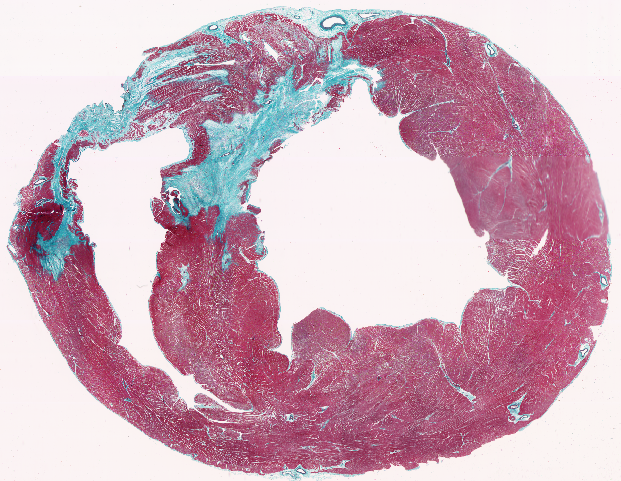
\includegraphics[width=\textwidth]{figures/Gip4_histology}
    \caption{Histology of a slice of infarcted heart nb 4}
    \label{fig:histology_pig_4}
\end{figure}

\section{Source of input data}

The data we have been using are DT-MRI of porcine hearts, both healthy for comparison and infarcted. We have had access to 10 hearts including 2 healthy. For every infarcted heart, the imaging process took place 6 weeks after infarct and histology was done after that for some of the cases - as it is an expensive process - which allows us to compare our observations to the ground truth. Here is an overview of the data we had access to and its usability:

\begin{center}
    \begin{tabular}{|c | c | c | c|} 
         \hline
         Heart (Acquisition Date) & Infarcted or Healthy & Region of infarct \\
         \hline
         2 & Infarcted & Left Circumflex artery (LCX) \\ 
         \hline
         4 & Infarcted & Left Anterior Descending (LAD) \\
         \hline
         5 & Infarcted & LCX \\
         \hline
         6 & Infarcted & LCX \\
         \hline
         7 & Infarcted & Rigth Coronary Artery (RCA) \\ 
         \hline
         17 & Infarcted & Bad quality \\
         \hline
         18 & Infarcted & Bad quality \\
         \hline
         23 & Infarcted & Unreadable \\
         \hline
         25 & Healthy & - \\
         \hline
         28 & Healthy & Too Noisy \\
         \hline
    \end{tabular}
\end{center}

\section{Quality of our data}

For a better and more accurate analysis of our results, we will focus mostly on the best quality data (least noisy) we had access to and fortunately those include one control heart (\#5: \ref{fig:pig25}) and 5 infarcted hearts (\#2: \ref{fig:pig2}, \#4: \ref{fig:pig4}, \#5: \ref{fig:pig5}, \#6: \ref{fig:pig6}, \#7: \ref{fig:pig7}). \\
Due to the imaging technology used, and to the fact that a fairly low Tesla intensity was used to acquire this data (1.5T), a good amount of noise is present in the raw data. We have taken advantage of the knowledge on the type of noise (Rician noise) that is present in MRI-acquired data to apply non-local denoising strategies which are a bit expensive in time but can smooth rather efficiently and not by too much the data to be able to have a better readability of the fiber orientation without oversmoothing. This prevents this strategy from smoothing even regions where the data is chaotic due to the infarct or proximity to the boundary and not only because of noise issues from acquisition. A fine tuning of the smoothing strategy allowed us to get good quality datasets without removing relevant information in the regions of interest around the infarcts.

\section{Usage of MedInria software to read the DICOMs}

We took the advantage of the MedInria tool to load the DICOM images, process the data through the Rician denoising method and finally use their Diffusion Tensor Imaging tool to compute the value of the tensor matrix \ref{diffusion_tensor_matrix} at each voxel location in the heart. \\
From the tensor matrices at every location, we were easily able to compute the fiber orientation at every location with a potential flip in the sense of the vector. Cylindrical consistency was used to enforce a consistent sense throughout the heart. \\
Once we have the fiber orientation at every voxel, we can use our previous work to compute the connection forms and get an approximative appreciation of the quality of the fitting, depending on hyper parameters that have to be fine tuned by mostly on the coherence of the underlying data. % Experimental Setup

%\newcommand{\degree}{^{\circ}}

\chapter{Results and Discussion}

We used an established Rician smoothing method to deal with noise in the diffusion images \cite{wiest2008rician}. This is a type of non-local smoothing technique which uses voxel to voxel similarity to guide the smoothing process. In general the parameters for this filtering method must be tuned to prevent oversmoothing, which can happen for instance if the weight is not sufficiently penalized when the similarity is not high enough. We used the publicly available MedInria software to carry out the filtering, and then to reconstruct the diffusion tensor from the raw diffusion weighted scans, from which fiber orientations were extracted as the first principal eigen vector. In practice we used a threshold on the FA map as a mask to restrict further processing.

\section{Quantitative Results}

\begin{figure}
    \centering
    \begin{subfigure}{1\textwidth}
        \centering
        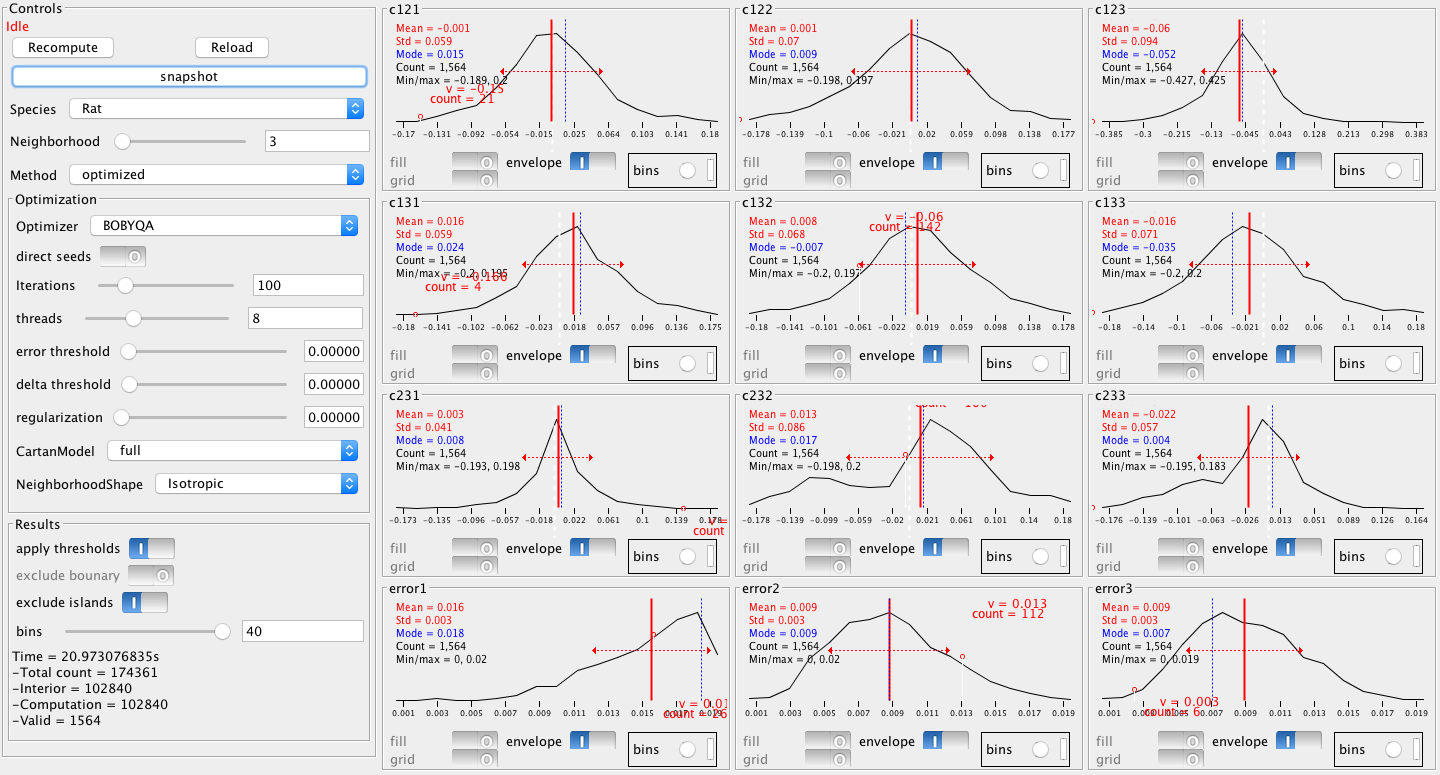
\includegraphics[width=\textwidth]{figures/histogram_pig6_no_smooth}
        \caption{Without any smoothing}
        \label{fig:histogram_pig6_no_smooth}
    \end{subfigure}
    \begin{subfigure}{1\textwidth}
        \centering
        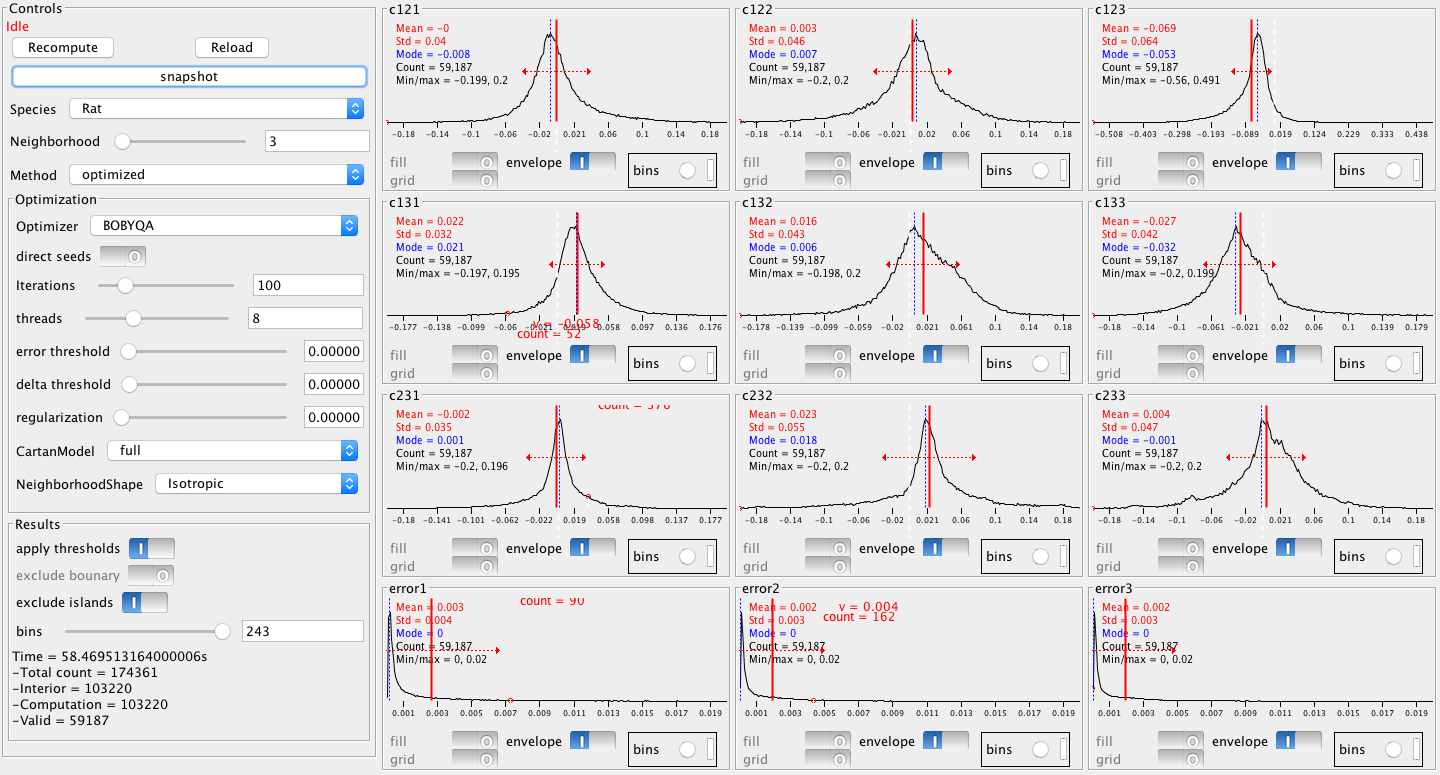
\includegraphics[width=\textwidth]{figures/histogram_pig6_smooth}
        \caption{With Rician smoothing}
        \label{fig:histogram_pig6_smooth}
    \end{subfigure}
    \caption{Histograms of error of fit and connection form parameters for pig \# 6}
    \label{histo_pig6}
\end{figure}

Given the association between ADC and our error of frame fit, it is natural to compare these measures quantitatively throughout the myocardium. We did so for the 5 infarcted porcine hearts we analyzed by computing Dice coefficients to describe the overlap, in the following manner:

For the same heart let A be the set of voxels with ADC value > 0.6 and let B be the set of voxels with error of fit $> 15 \degree$. We computed the standard Dice coefficient $\frac{A \cap B}{A \cup B}$ as well as a modified coefficient $\frac{A \cap B}{A}$.
\begin{table}
    \centering
    \begin{tabular}{|c | c | c |}
         \hline
         Heart & $\frac{A \cap B}{A \cup B}$ & $\frac{A \cap B}{A}$ \\
         \hline
         2 & 0.40 & 0.80 \\ 
         \hline
         4 & 0.43 & 0.89 \\
         \hline
         5 & 0.47 & 0.76 \\
         \hline
         6 & 0.46 & 0.87 \\
         \hline
         7 & 0.27 & 0.94 \\ 
         \hline
    \end{tabular}
    \caption{Dice and modified coefficients for infarcted hearts}
\end{table}

These results demonstrate that typically over 80\% of the locations with increased diffusion also yield a high error of fit using our frame fitting method, due to the loss of geometric coherence of fiber orientations. However there are additional locations where fiber orientations are not smooth, typically at the linings of the heart wall, or near the edges of a collapsing and narrow right ventricle. These are picked up by our error of fit measure but not by the ADC measure, likely because there is no increase in collagen there.

\subsection{Histograms of connection forms} \label{histogram_section}

Here are examples of the histograms that we computed on the entire heart for every usable example that we had. The histogram in Fig. \ref{fig:histogram_pig6_smooth} gives us information on the distribution of $c_{i,j,k}, \forall (i, j, k) \in [1, 3]^3$ and the distribution of the error of fit for each frame axis $\mathbf{f}_1, \mathbf{f}_2$ and $\mathbf{f}_3$.

In this thesis we will focus on the most commonly used parameter for comparison, the helix angle $c_{1,2,3}$. Our tool gives us the mean and the mode (value most represented) of this value through the whole heart. As we have a Gaussian distribution of these values the mode is relevant and helping as it will represent mostly fibers in the core of the heart wall and not take into account (as the mean value does) extreme values that can occur on the boundaries of the heart wall.

The papillary muscles, to name only one side effect, which are mostly aligned in a top-down direction along the long axis, can have non negligible effect on the $c_{1,2,3}$ value and they are difficult to remove from our model as it can be difficult to determine where they start exactly and which layer should then be kept and which should be considered as papillary muscle and therefore removed.

In the table we regroup the results we obtained from all relevant datasets and analyze the total helix angle in degrees that we obtain the following way (where 57.3 is the conversion from rad to $\degree$):
\begin{equation}
    \text{total helix angle} = c_{1,2,3}\cdot \text{\#voxels}\cdot 57.3
\end{equation}
The values that we get are close to the theoretical value of $120\degree$ reported in the literature \cite{piuzephd}.

\begin{table}
    \centering
    \begin{tabular}{|c | c | c | c| c| c|} 
         \hline
         Heart & \shortstack{Thickness \\ (\# voxels)} & \shortstack{$c_{1,2,3}$ mean \\ rad/voxel} & \shortstack{$c_{1,2,3}$ mode \\ rad/voxel} & \shortstack{Total helix angle \\ (using mean)} & \shortstack{Helix angle \\ (using mode)}\\
         \hline
         2 & 40 & -0.066 & -0.025 & -151.2$\degree$ & -57.3$\degree$ \\ 
         \hline
         4 & 45 & -0.084 & -0.047 & -216.6$\degree$ & -121.2$\degree$ \\
         \hline
         5 & 30 & -0.048 & -0.020 & -82.5$\degree$ & -34.38$\degree$ \\
         \hline
         6 & 30 & -0.069 & -0.053 & -118.6$\degree$ & -91.1$\degree$ \\
         \hline
         7 & 45 & -0.077 & -0.053 & -198.5$\degree$ & -136.6$\degree$ \\ 
         \hline
         25 & 35 & -0.072 & -0.034 & -144.4$\degree$ & -68.2$\degree$ \\
         \hline
    \end{tabular}
    \caption{Total helix angle using our connection form parameters}
\end{table}


\section{Qualitative Results}

\subsection{Importance of the filtering from the fibers...}

In topview figures \ref{fig:pig4_topviews} and a more transverse view where the helix angle is easier to visualize in Fig. \ref{fig:pig4_helix}, we have a first glimpse at the difference of the fiber orientation and cohesion before and after smoothing the raw data through a Rician filter, which is the appropriate filtering method when dealing with DMRI data.

The region shown in figures \ref{fig:pig4_helix_no_smooth} and \ref{fig:pig4_helix_smooth} is a region away from the infarct where we should see a smooth turning of fibers. This region corresponds to the top-right region of the same slice presented in figures \ref{fig:pig4_topview_no_smooth} and \ref{fig:pig4_topview_smooth}.

Tracing fibers from raw data leads to an extremely noisy data from which it is hard to infer any general structure, which we will see in Fig. \ref{fig:histogram_pig6_no_smooth}. Indeed the low magnetic field value (1.5T) is one of the reasons why the data is not of the highest quality, as well as the low number of iterations in the acquisition process.

Thanks to the Rician smoothing it is again possible to guess the helix angle turning from outer wall to inner wall although this is still not perfect, as we want to keep as much information as possible with using the lightest filtering possible.

\begin{figure}[h!]
    \centering
    \begin{subfigure}{.48\textwidth}
        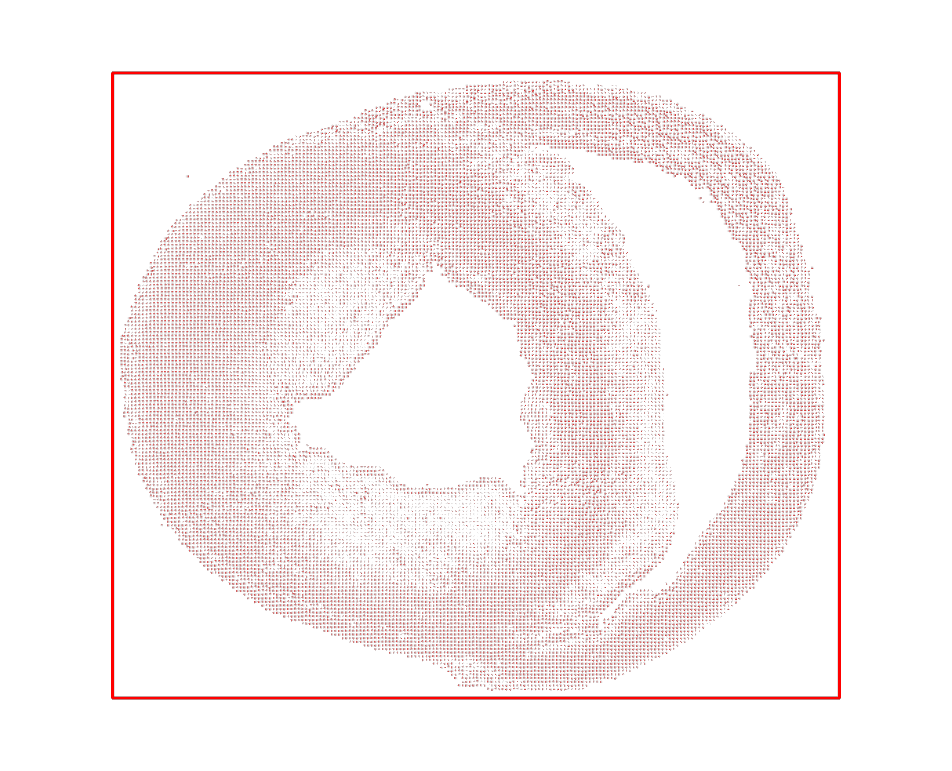
\includegraphics[width=\textwidth]{figures/pig4_topview_no_smooth}
        \caption{Without any smoothing}
        \label{fig:pig4_topview_no_smooth}
    \end{subfigure}
    \begin{subfigure}{.48\textwidth}
        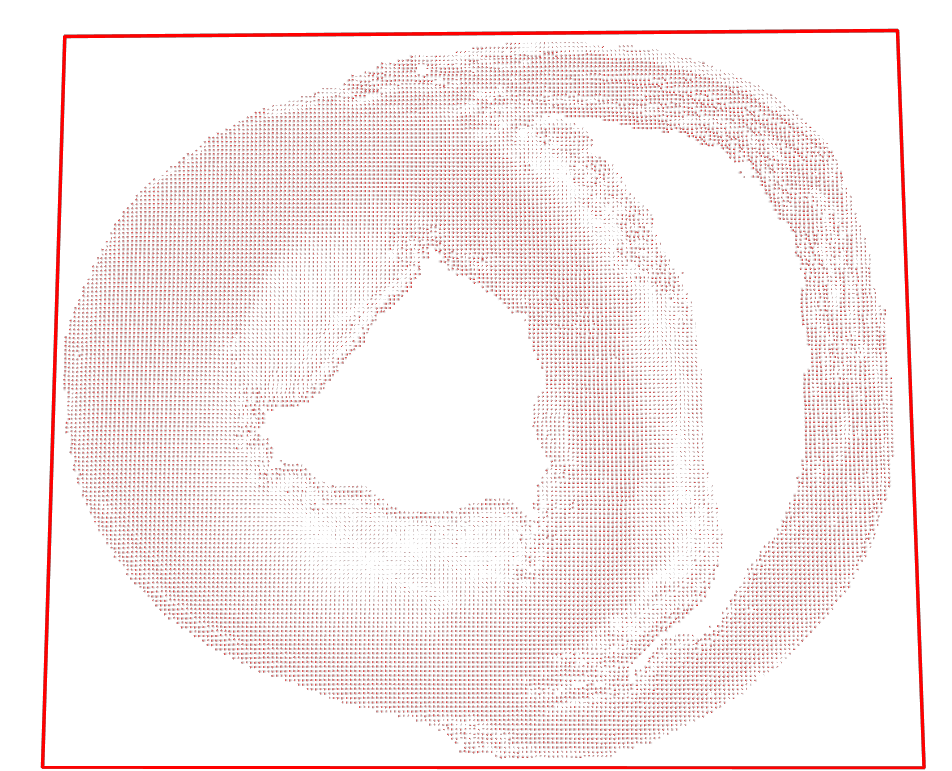
\includegraphics[width=\textwidth]{figures/pig4_topview_smooth}
        \caption{With Rician smoothing}
        \label{fig:pig4_topview_smooth}
    \end{subfigure}
    \caption{Top view of heart fibers for pig 4}
    \label{fig:pig4_topviews}
    \begin{subfigure}{.48\textwidth}
        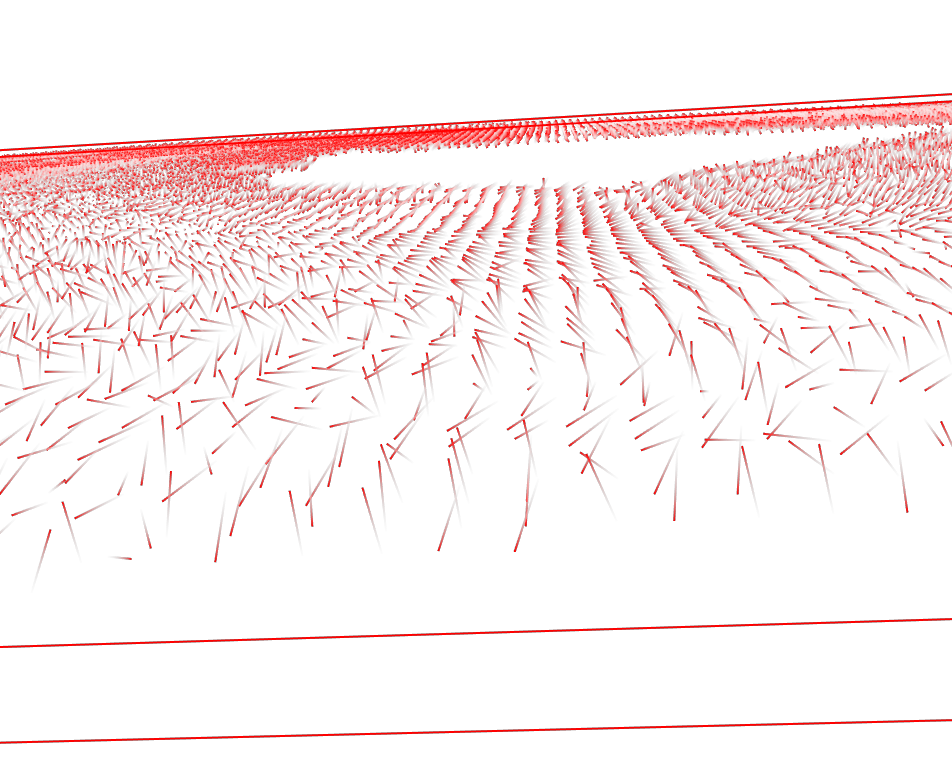
\includegraphics[width=\textwidth]{figures/pig4_helix_no_smooth}
        \caption{Without any smoothing}
        \label{fig:pig4_helix_no_smooth}
    \end{subfigure}
    \begin{subfigure}{.48\textwidth}
        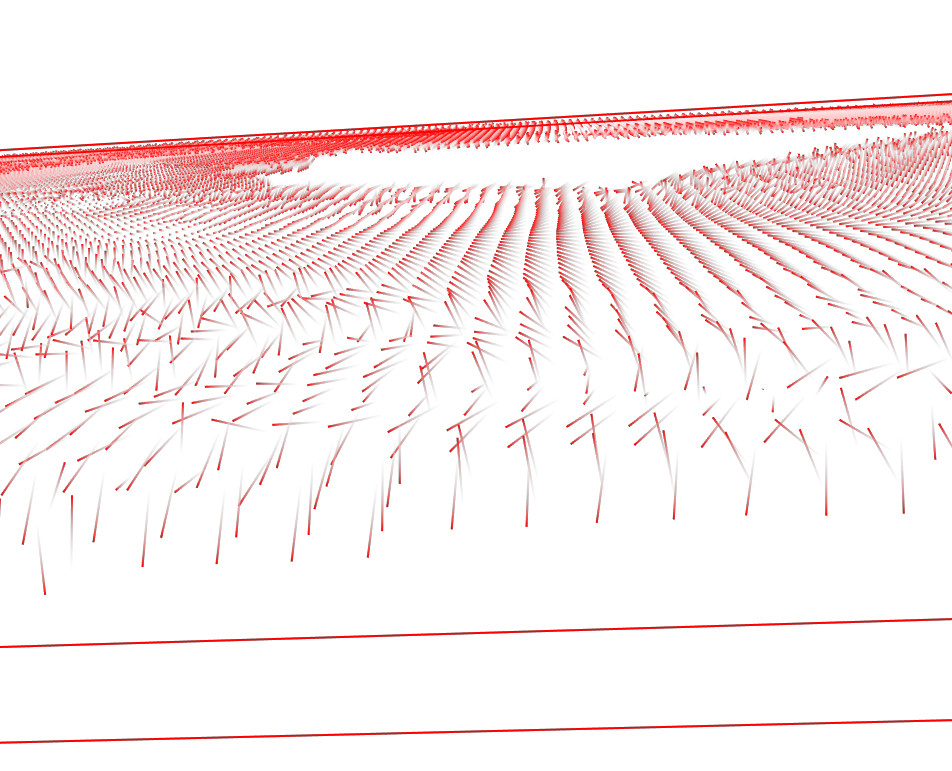
\includegraphics[width=\textwidth]{figures/pig4_helix_smooth}
        \caption{With Rician smoothing}
        \label{fig:pig4_helix_smooth}
    \end{subfigure}
    \caption{View of the helix angle of heart fibers for pig 4}
    \label{fig:pig4_helix}
\end{figure}

\subsection{...To the tractography and fitting process}

Using the fiber orientation that we can get from the computed tensor matrix, we can run tractography on our results. This process gives us an idea of how fibers should be wrapped around the heart and work together in the muscle structure. Looking at the tractography run on the raw data on Fig. \ref{fig:pig4_tracto_no_smooth} it is hard to see where the infarct would be by just looking at the tracing of existing fibers and trying to infer their direction. The infarct region, as explained in \cite{wu2007mr}, should be the region with the least coherence in its fiber directions whereas regions remote from the infarct should not be affected in their structure.

\begin{figure}[h!]
    \centering
    \begin{subfigure}{.48\textwidth}
        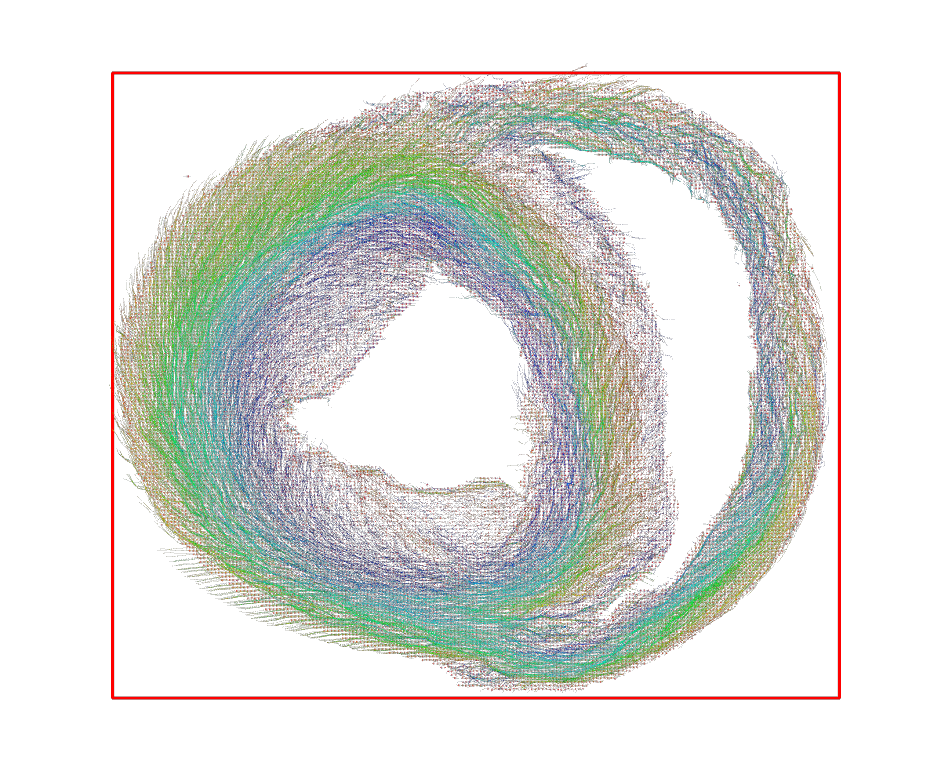
\includegraphics[width=\textwidth]{figures/pig4_topview_tracto_no_smooth}
        \caption{Without any smoothing}
        \label{fig:pig4_tracto_no_smooth}
    \end{subfigure}
    \begin{subfigure}{.48\textwidth}
        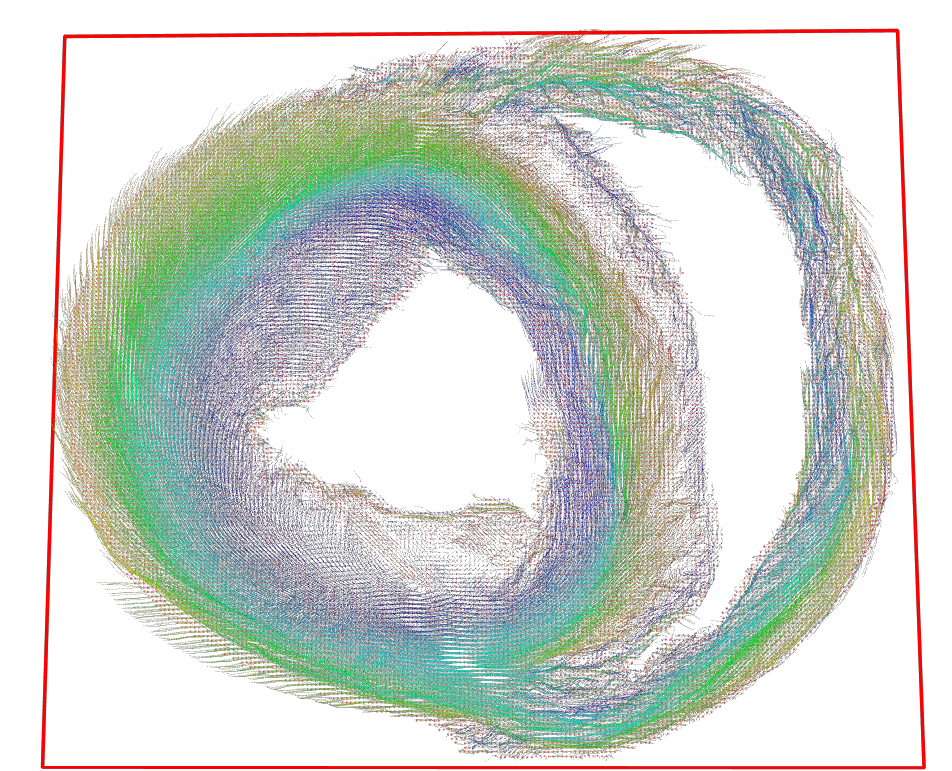
\includegraphics[width=\textwidth]{figures/pig4_topview_tracto_smooth}
        \caption{With Rician smoothing}
        \label{fig:pig4_tracto_smooth}
    \end{subfigure}
    \caption{Tractography of heart fibers for pig 4}
    \label{fig:pig4_tractos}
\end{figure}

Looking at the tractography run on the Rician smoothed data in Fig. \ref{fig:pig4_tracto_smooth} on the other hand gives a clear hint on the region where the infarct is present (LAD) whereas remote regions do not seem affected by this and wrap smoothly around the heart.

Finally, looking at histograms in figures \ref{fig:histogram_pig6_no_smooth} and \ref{fig:histogram_pig6_smooth} we can get from our procedure to look at statistics on the visualized information presented, we see several clear indications that smoothing will be a capital step in our further analysis of our datasets:
\begin{enumerate}
    \item Shape of Gaussians we get from the datasets. The center is much better defined in for the smoothed data in Fig. \ref{fig:histogram_pig6_smooth} as well as overall shape which is less spiky
    \item The number of voxels that count in our computations: from $1564$ with raw unfiltered data in Fig. \ref{fig:histogram_pig6_no_smooth} to $59187$ after the Rician filter in Fig. \ref{fig:histogram_pig6_smooth}
\end{enumerate}
The number of voxels that count in our computations is the number of voxels where we could converge to a value of connection form matrix $(c_{i, j, k})_{(i, j, k) \in \mathbb{R}^3}$. Voxels where we could not converge to a value after a given number of iterations were discarded in the histogram to limit the noise importance in the final observations.

\subsection{Error of fit vs ADC and FA}

\begin{figure}[h!]
    \centering
    \begin{subfigure}{.31\textwidth}
        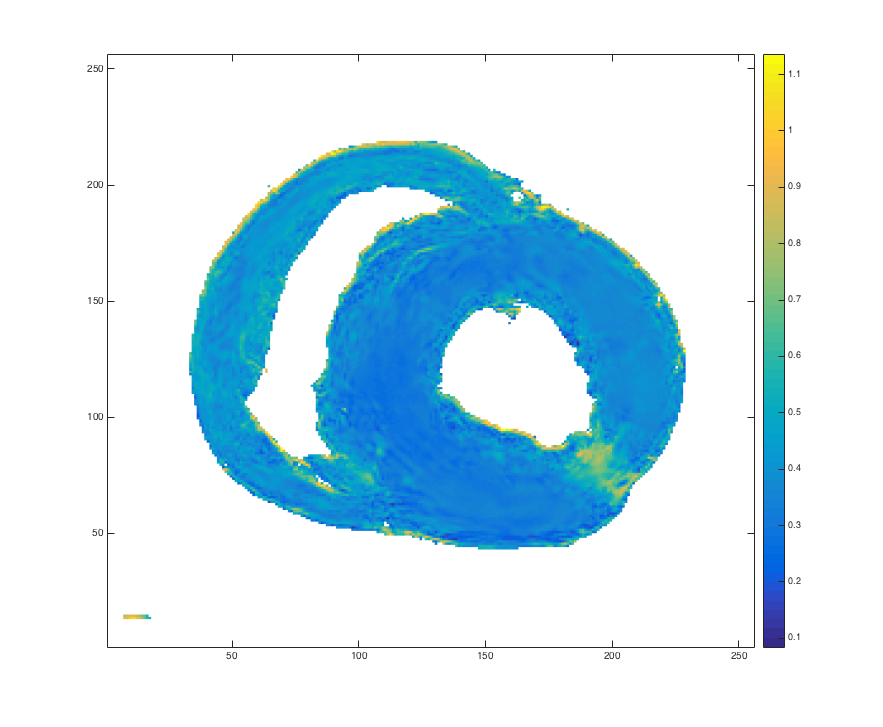
\includegraphics[width=\textwidth]{figures/pig2_adc_31}
        \caption{ADC map}
        \label{fig:pig2_adc}
    \end{subfigure}
    \begin{subfigure}{.31\textwidth}
        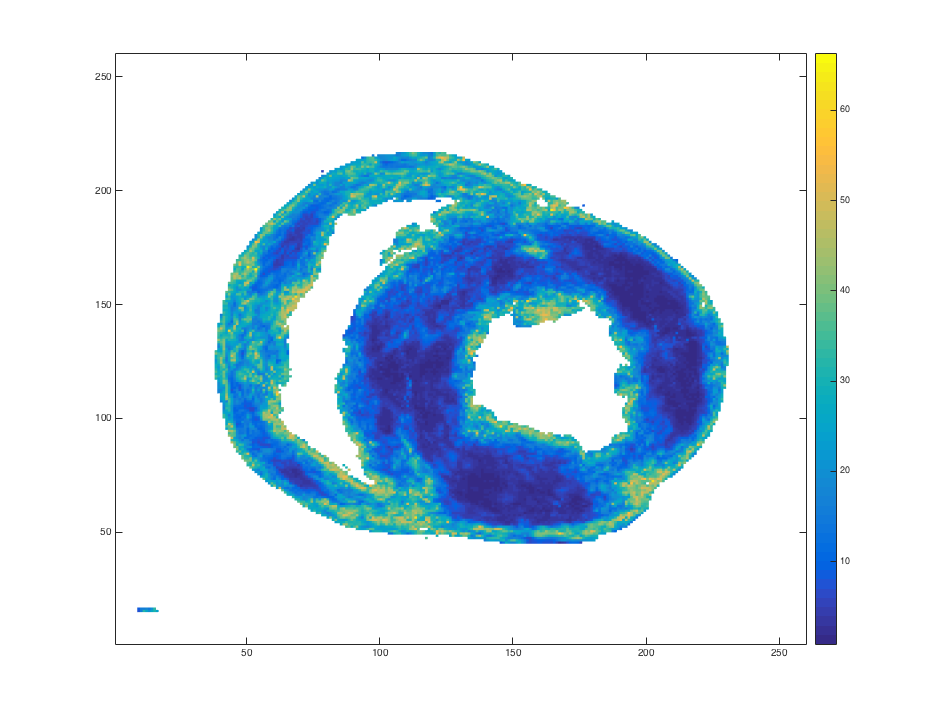
\includegraphics[width=\textwidth]{figures/pig2_err_31}
        \caption{Error of fit}
        \label{fig:pig2_err}
    \end{subfigure}
    \begin{subfigure}{.31\textwidth}
        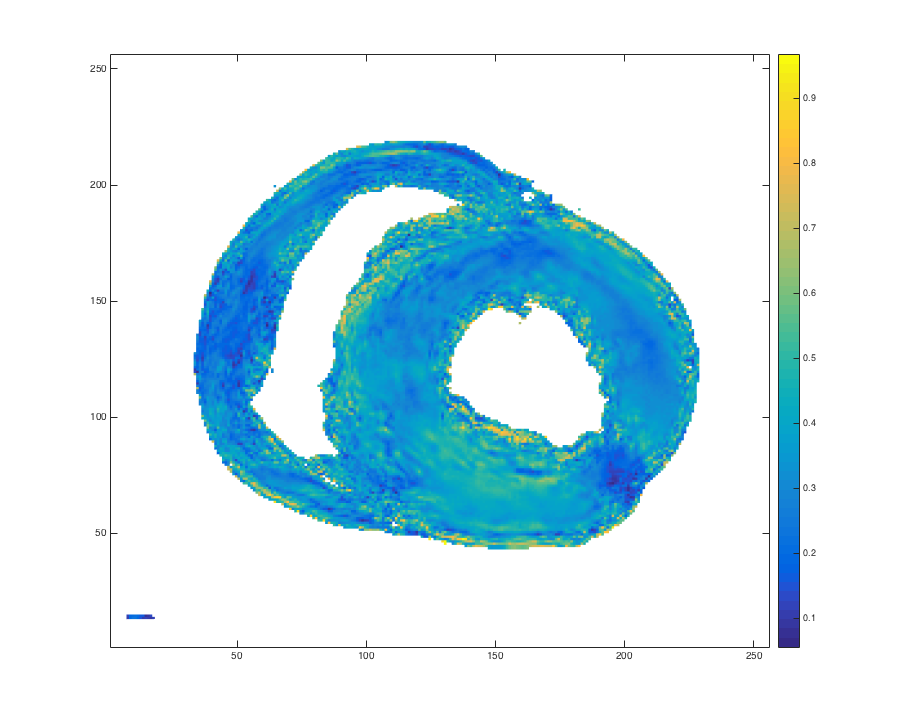
\includegraphics[width=\textwidth]{figures/pig2_fa_31}
        \caption{FA map}
        \label{fig:pig2_fa}
    \end{subfigure}
    \caption{Pig 2: Error of fit computed using our framework compared to ADC and FA map}
    \label{fig:pig2}


    \begin{subfigure}{.31\textwidth}
        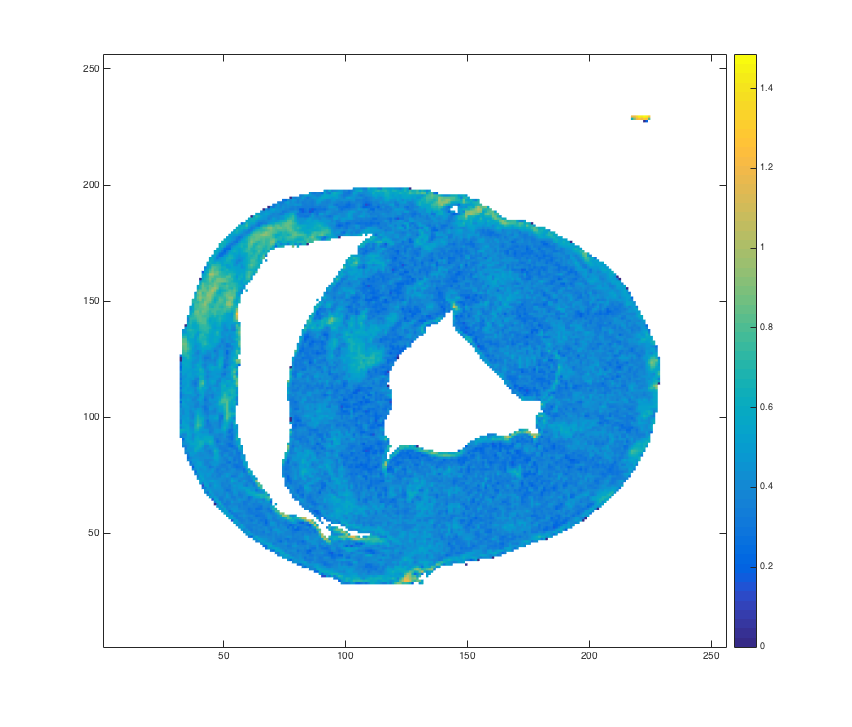
\includegraphics[width=\textwidth]{figures/pig4_adc_21}
        \caption{ADC map}
        \label{fig:pig4_adc}
    \end{subfigure}
    \begin{subfigure}{.31\textwidth}
        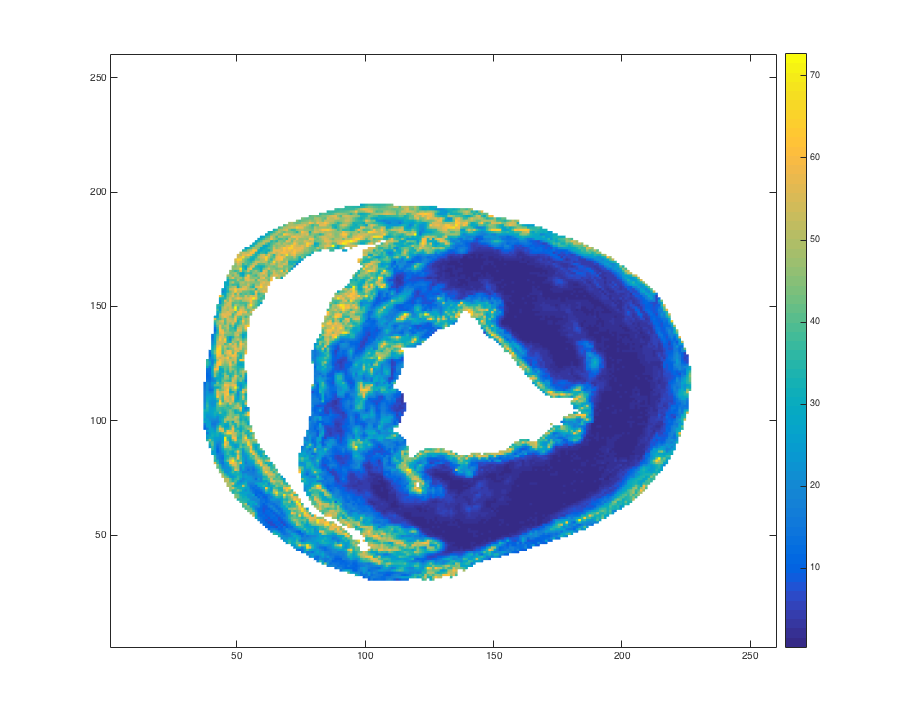
\includegraphics[width=\textwidth]{figures/pig4_err_21}
        \caption{Error of fit}
        \label{fig:pig4_err}
    \end{subfigure}
    \begin{subfigure}{.31\textwidth}
        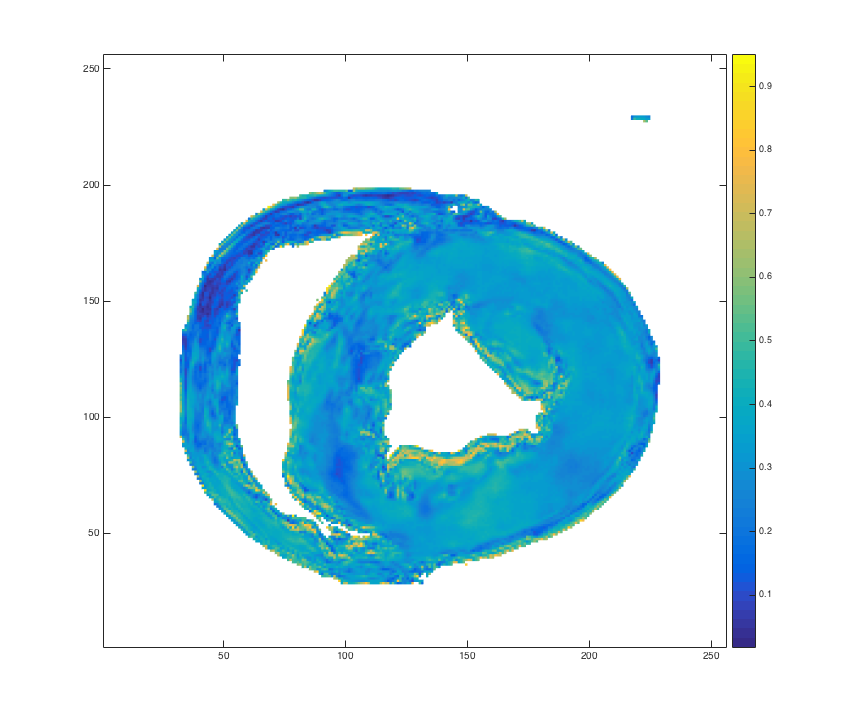
\includegraphics[width=\textwidth]{figures/pig4_fa_21}
        \caption{FA map}
        \label{fig:pig4_fa}
    \end{subfigure}
    \caption{Pig 4}
    \label{fig:pig4}
    
    \begin{subfigure}{.31\textwidth}
        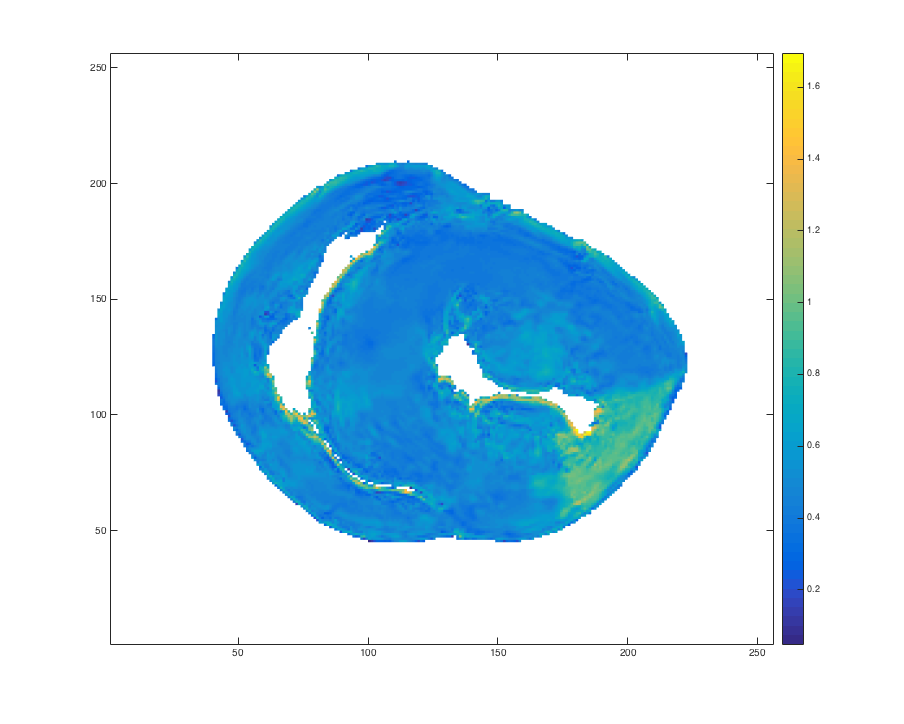
\includegraphics[width=\textwidth]{figures/pig5_adc_22}
        \caption{ADC map}
        \label{fig:pig5_adc}
    \end{subfigure}
    \begin{subfigure}{.31\textwidth}
        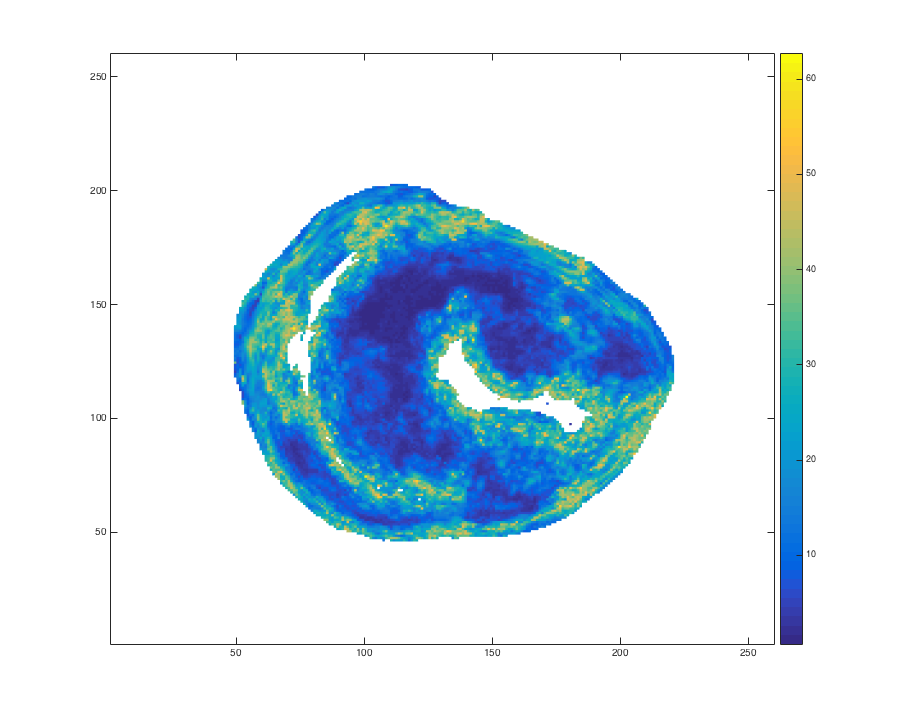
\includegraphics[width=\textwidth]{figures/pig5_err_22}
        \caption{Error of fit}
        \label{fig:pig5_err}
    \end{subfigure}
    \begin{subfigure}{.31\textwidth}
        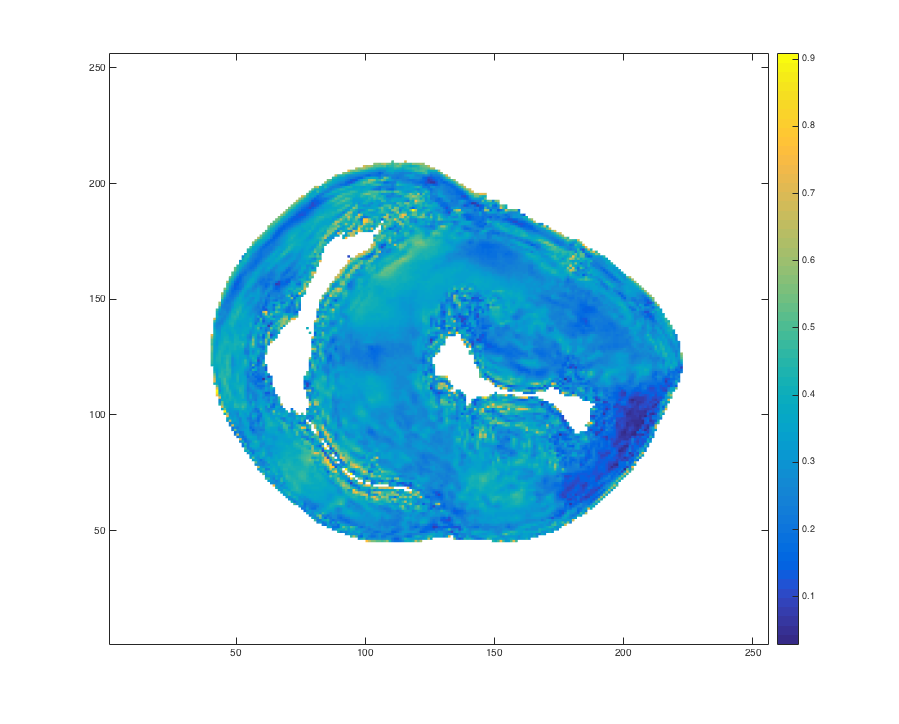
\includegraphics[width=\textwidth]{figures/pig5_fa_22}
        \caption{FA map}
        \label{fig:pig5_fa}
    \end{subfigure}
    \caption{Pig 5}
    \label{fig:pig5}
\end{figure}
    
\begin{figure}[h!]
    \centering
    \begin{subfigure}{.31\textwidth}
        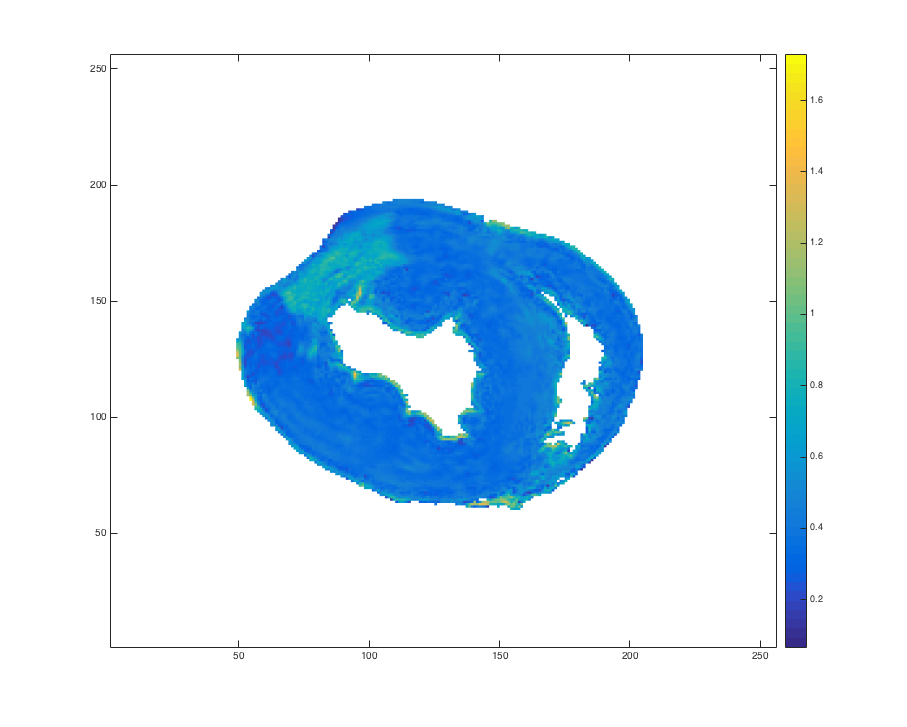
\includegraphics[width=\textwidth]{figures/pig6_adc_24}
        \caption{ADC map}
        \label{fig:pig6_adc}
    \end{subfigure}
    \begin{subfigure}{.31\textwidth}
        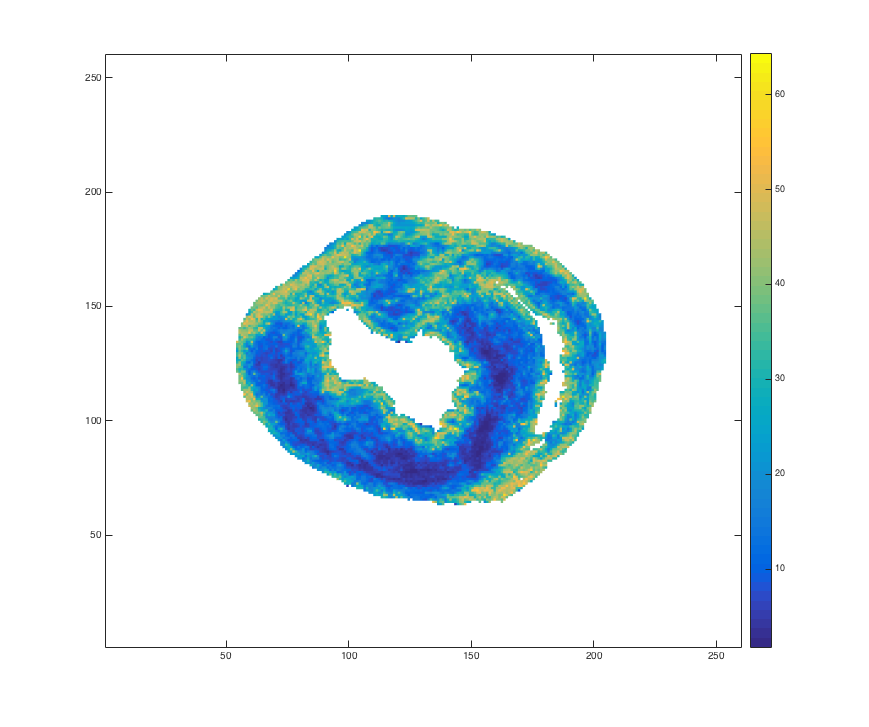
\includegraphics[width=\textwidth]{figures/pig6_err_24}
        \caption{Error of fit}
        \label{fig:pig6_err}
    \end{subfigure}
    \begin{subfigure}{.31\textwidth}
        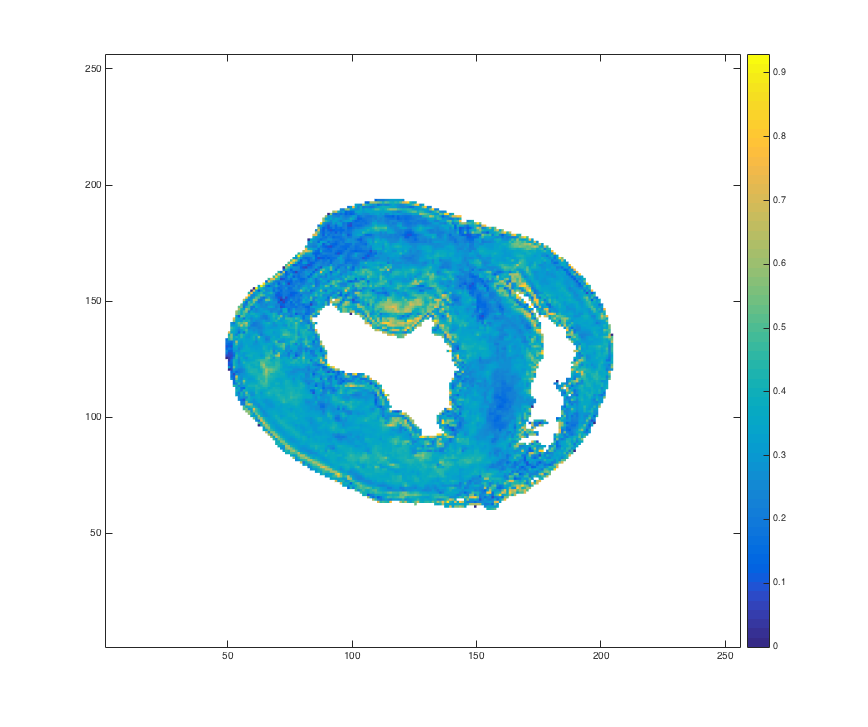
\includegraphics[width=\textwidth]{figures/pig6_fa_24}
        \caption{FA map}
        \label{fig:pig6_fa}
    \end{subfigure}
    \caption{Pig 6}
    \label{fig:pig6}
    
    \begin{subfigure}{.31\textwidth}
        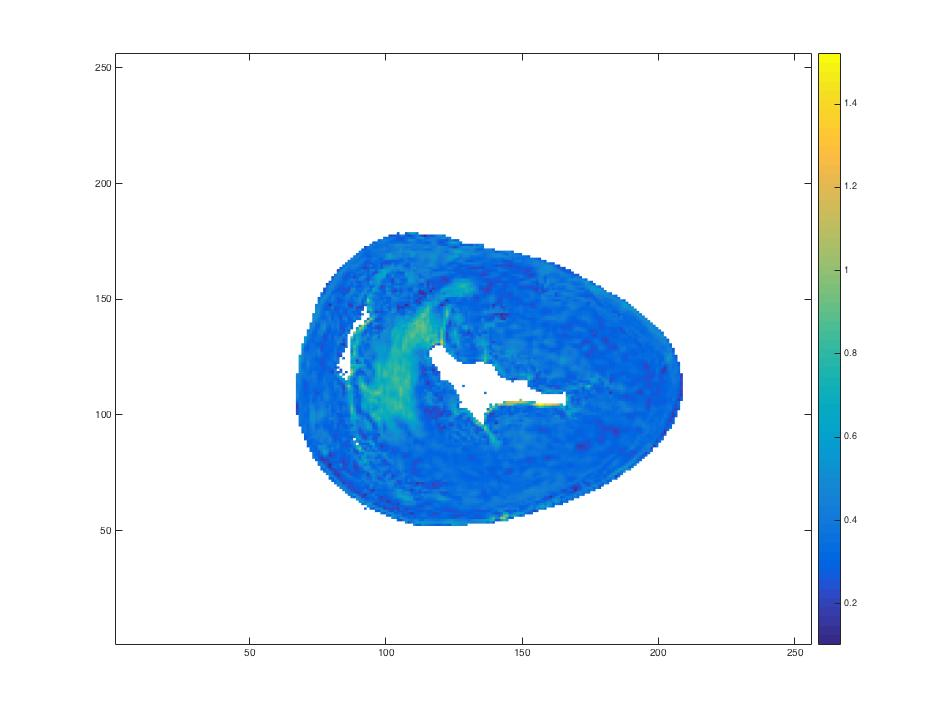
\includegraphics[width=\textwidth]{figures/pig7_adc_14}
        \caption{ADC map}
        \label{fig:pig7_adc}
    \end{subfigure}
    \begin{subfigure}{.31\textwidth}
        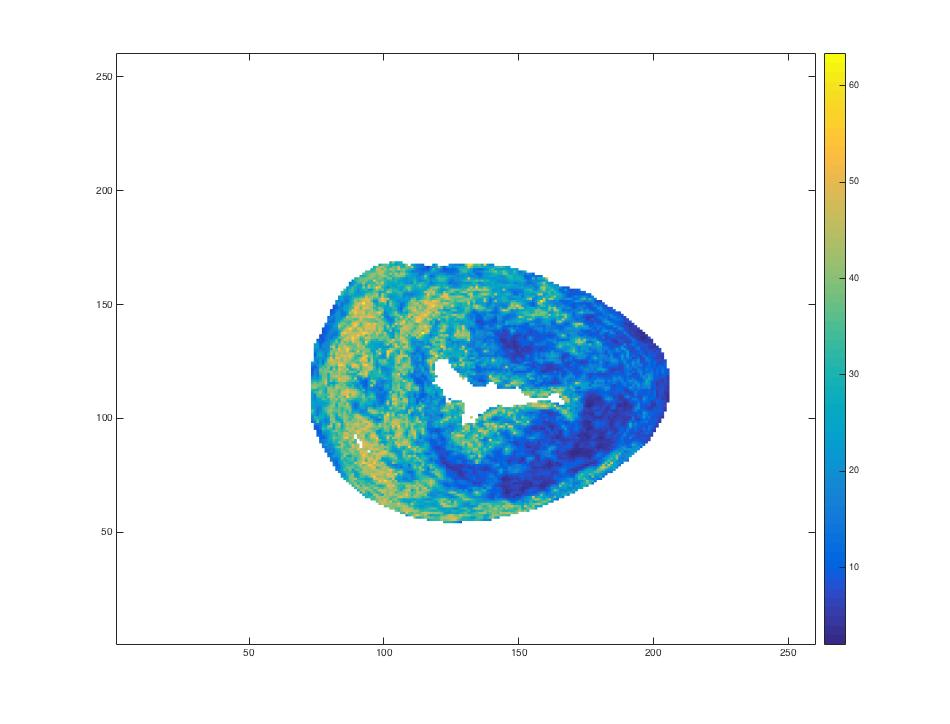
\includegraphics[width=\textwidth]{figures/pig7_err_14}
        \caption{Error of fit}
        \label{fig:pig7_err}
    \end{subfigure}
    \begin{subfigure}{.31\textwidth}
        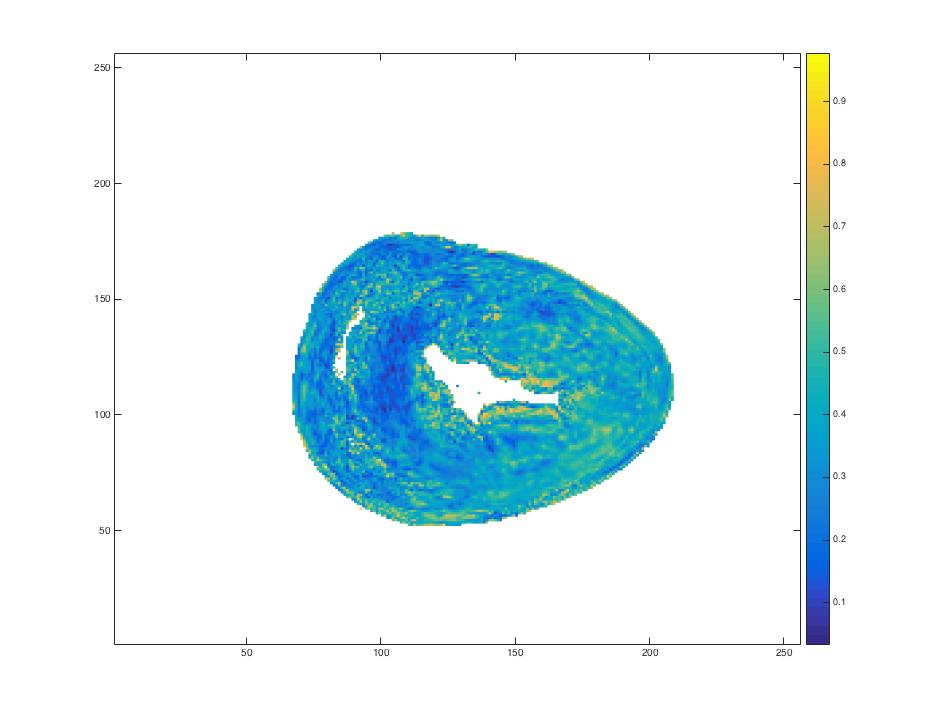
\includegraphics[width=\textwidth]{figures/pig7_fa_14}
        \caption{FA map}
        \label{fig:pig7_fa}
    \end{subfigure}
    \caption{Pig 7}
    \label{fig:pig7}
    
    \begin{subfigure}{.31\textwidth}
        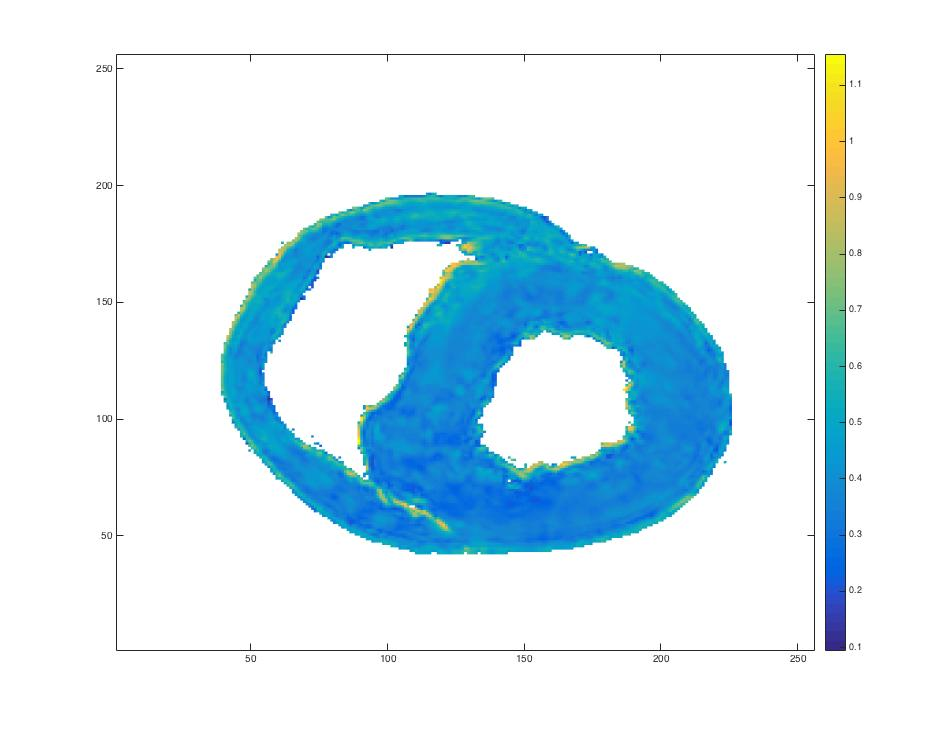
\includegraphics[width=\textwidth]{figures/pig25_adc_30}
        \caption{ADC map}
        \label{fig:pig25_adc}
    \end{subfigure}
    \begin{subfigure}{.31\textwidth}
        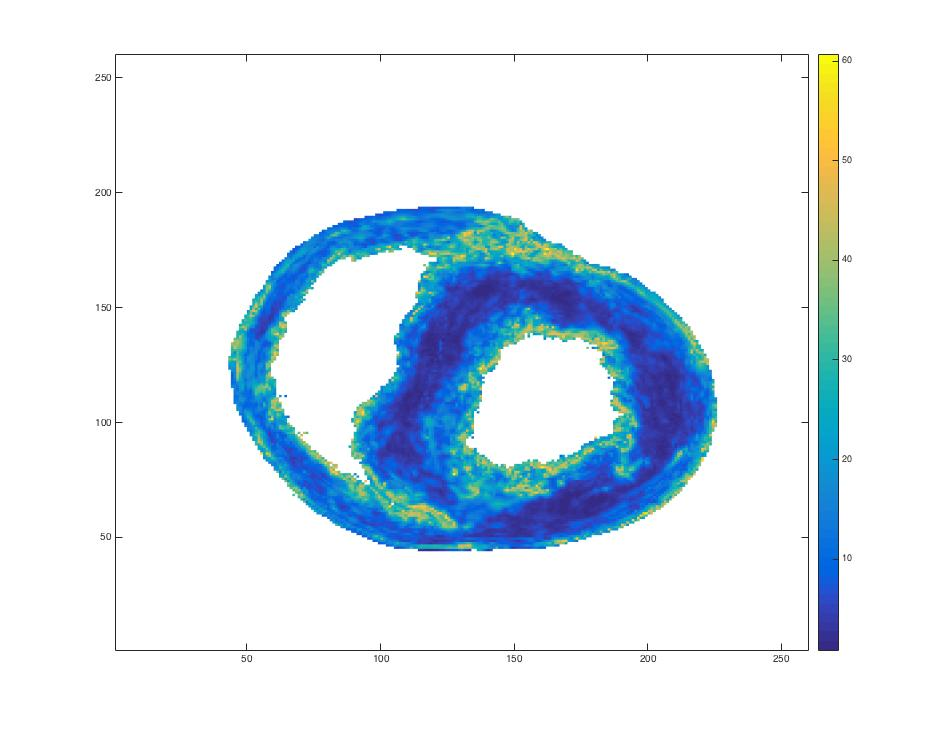
\includegraphics[width=\textwidth]{figures/pig25_err_30}
        \caption{Error of fit}
        \label{fig:pig25_err}
    \end{subfigure}
    \begin{subfigure}{.31\textwidth}
        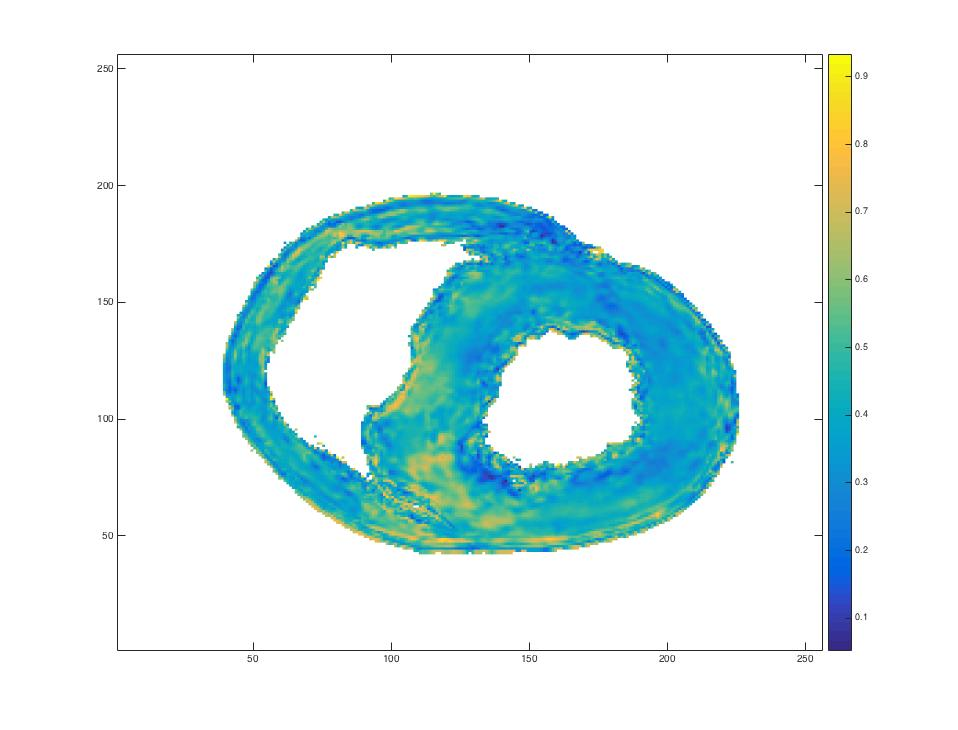
\includegraphics[width=\textwidth]{figures/pig25_fa_30}
        \caption{FA map}
        \label{fig:pig25_fa}
    \end{subfigure}
    \caption{Pig 25}
    \label{fig:pig25}
\end{figure}

These figures give us a good understanding and overview of how the error of fit can provide supplementary information compared to what the ADC and FA map can give us.

If we focus on the first example - Fig. \ref{fig:pig2}, we can clearly see in the ADC map shown in Fig. \ref{fig:pig2_adc} the region of the infarct where the value is the highest (yellow region); and it really gives the impression of a scar region that contains almost only collagen and no fibrous tissue whatsoever given the apparent anisotropy. But if we look at the FA map presented in Fig. \ref{fig:pig2_fa} we can start wondering if there is not a region close to the endocardium where fibers have either resisted or been reconstructed after the infarct in this region.

As for the error of fit, it gives a clear indication of the existence of layers of fibers near the endocardium that still makes the connection with the rest of the heart possible and the contraction, even if badly hindered by the infarct and loss of muscle fibers, still possible.

This arrangement of the surviving fibers as described in the literature overviewed in Section \ref{surviving_fibers} is also clearly visible in the examples displayed in Fig. \ref{fig:pig4} and \ref{fig:pig5}.

The example Fig. \ref{fig:pig6} is also a very interesting sample to compare our method to, and it shows that in some cases as mentioned in \cite{ursell1985structural}, intramural muscles seem to be completely absent in this case and can gravely hinder the contraction of the heart.

Our approach seems to be more tolerant in the exhibition of surviving fibers in the infarct region and in some cases show how CR can make the infarct region still a little contractile.

The last provided example - Fig. \ref{fig:pig25} - is used as a control healthy heart to make sure of the extent to which we can use our results. We can clearly see in this healthy example that the error of fit is low pretty much everywhere, except in regions near the heart wall (endothilial and epithilial) and the region where the Left Ventricle (LV) and the Right Ventricle (RV) connect to each other. This is due to difficulty in our method to compute connection forms in areas where fibers tend to go in different directions, depending if they work towards the LV contraction, the RV contraction or else. Then the method performs less well to try to fit smoothly varying geometrical fiber structures.

\subsection{Discussion}

In all the examples seen in the previous section, locations where the ADC value is high are typically also ones where the error of fit is high, with regions of low error of fit being restricted to healthy tissue. In addition though, the error of fit is also consistently high at locations close to the epithelial and endothelial boundaries, signaling a loss in geometric coherence of fibers there. Curiously this phenomena is also seen at the borders of the healthy heart in Fig. \ref{fig:pig25_err}.

The error of fit shows information about the existence of surviving fibers in the infarct and border zone that can help the contractile function of the heart after the infarct. This is precious knowledge as it is a non-invasive way to qualify the capacity of the heart to keep beating and pumping blood to the body although the heart has suffered from an infarct. Further experiments could be made to support this analysis and show how the efficiency of an infarcted heart is related to the remaining fibers by conducting blood flow experiments before the imaging process.

Another very promising research topic would be to analyze the evolution of surviving fibers at different time frames after infarct, as we were limited to the datasets available which were all 6 weeks after infarct.
 % Experiment 1

%\chapter{Results and Discussion}

We used an established Rician smoothing method to combat noise in the diffusion images \cite{wiest2008rician}. This is a type of non-local smoothing technique which uses voxel to voxel similarity to guide the smoothing process. In general the parameters for this filtering method must be tuned to prevent oversmoothing, which can happen for instance if the weight is not sufficiently penalized when the similarity is not high enough. We used the publicly available MedInria software to carry out the filtering, and then to reconstruct the diffusion tensor from the raw diffusion weighted scans, from which fiber orientations were extracted as the first principal eigen vector. In practice we used a threshold on the FA map as a mask to restrict further processing.

\section{Qualitative Results}

\subsection{Importance of the filtering from the fibers...}

In topview figures \ref{fig:pig4_topviews} and a more transverse view where the helix angle is easier to visualize \ref{fig:pig4_helix}, we have a first glimpse at the difference of the fiber orientation and cohesion before and after smoothing the raw data through a Rician filter, which is the appropriate filtering method when dealing with DMRI data.\\
The region shown in figures \ref{fig:pig4_helix_no_smooth} and \ref{fig:pig4_helix_smooth} is a region away from the infarct where we should see a smooth turning of fibers. This region corresponds to the top-right region of the same slice presented in figures \ref{fig:pig4_topview_no_smooth} and \ref{fig:pig4_topview_smooth}.\\
Tracing fibers from raw data leads to an extremely noisy data from which it is hard to infer any general structure, which we will see in \ref{fig:histogram_pig6_no_smooth}. Indeed the low magnetic field value (1.5T) is one of the reasons why the data is not of the highest quality, as well as the low number of iterations in the acquisition process.\\
Thanks to the Rician smoothing it is again possible to guess the helix angle turning from outer wall to inner wall although this is still not perfect, as we want to keep as much information as possible with using the lightest filtering possible.

\begin{figure}
    \centering
    \begin{subfigure}{.48\textwidth}
        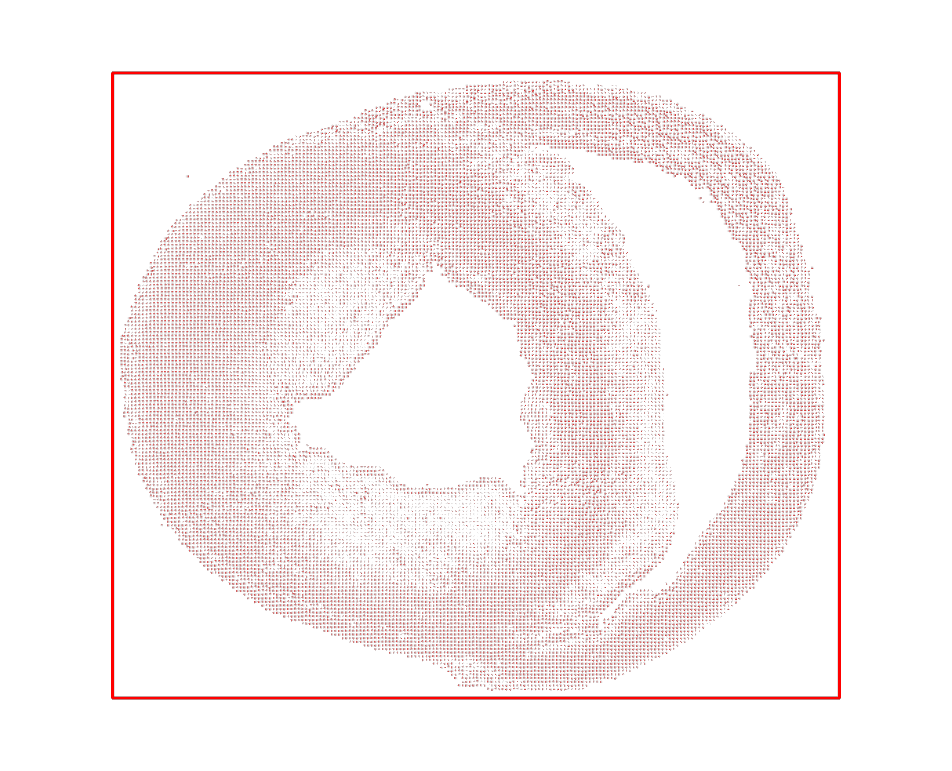
\includegraphics[width=\textwidth]{figures/pig4_topview_no_smooth}
        \caption{Without any smoothing}
        \label{fig:pig4_topview_no_smooth}
    \end{subfigure}
    \begin{subfigure}{.48\textwidth}
        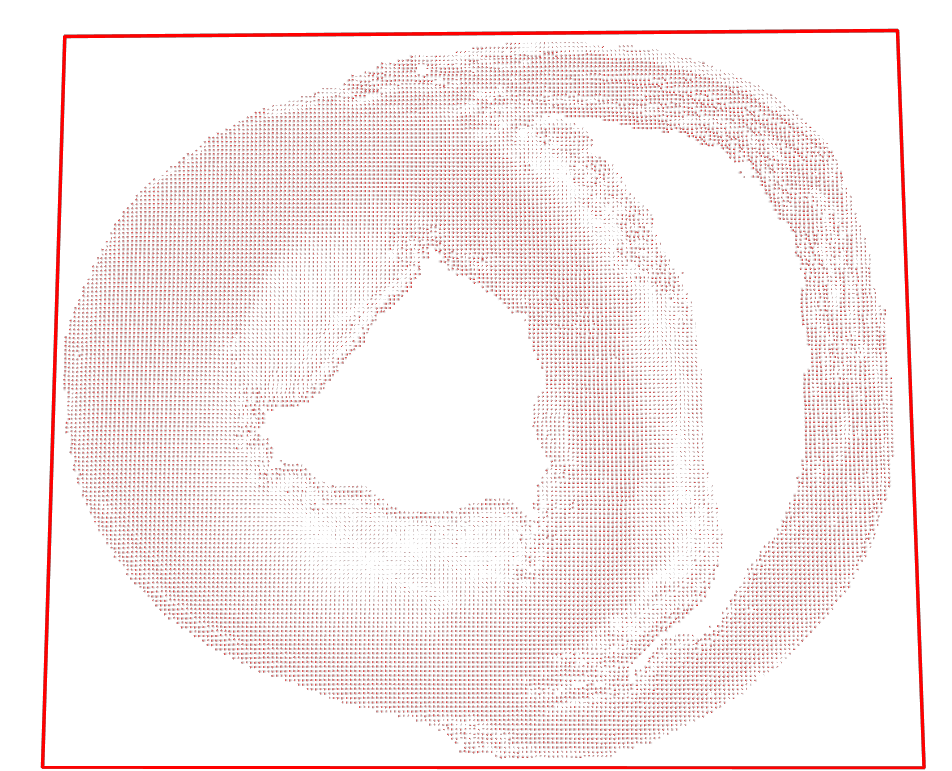
\includegraphics[width=\textwidth]{figures/pig4_topview_smooth}
        \caption{With Rician smoothing}
        \label{fig:pig4_topview_smooth}
    \end{subfigure}
    \caption{Top view of heart fibers for pig 4}
    \label{fig:pig4_topviews}
\end{figure}

\begin{figure}
    \centering
    \begin{subfigure}{.48\textwidth}
        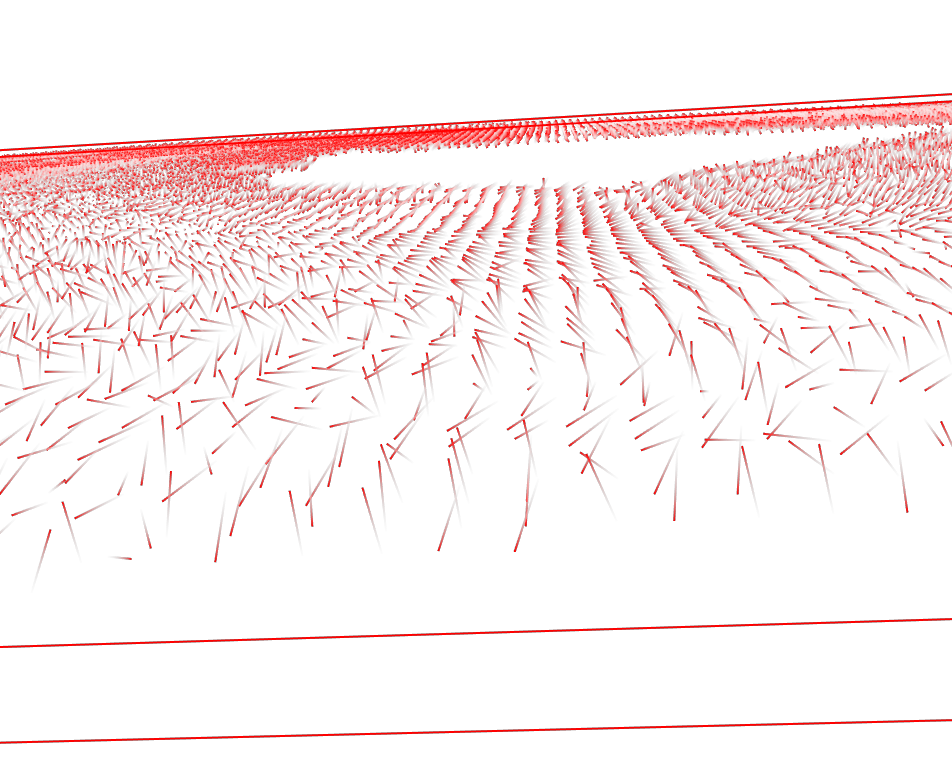
\includegraphics[width=\textwidth]{figures/pig4_helix_no_smooth}
        \caption{Without any smoothing}
        \label{fig:pig4_helix_no_smooth}
    \end{subfigure}
    \begin{subfigure}{.48\textwidth}
        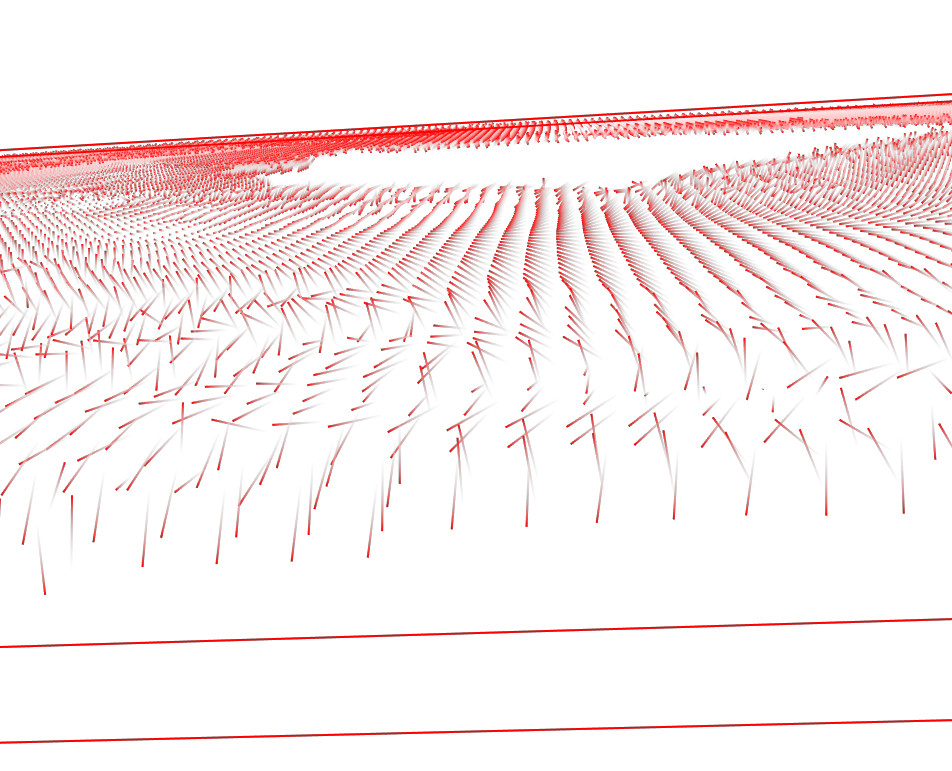
\includegraphics[width=\textwidth]{figures/pig4_helix_smooth}
        \caption{With Rician smoothing}
        \label{fig:pig4_helix_smooth}
    \end{subfigure}
    \caption{View of the helix angle of heart fibers for pig 4}
    \label{fig:pig4_helix}
\end{figure}

\subsection{...To the tractography and fitting process}

Using the fiber orientation that we can get from the computed tensor matrix, we can run tractography on our results. This process gives us an idea of how fibers should be wrapped around the heart and work together in the muscle structure. Looking at the tractography run on the raw data \ref{fig:pig4_tracto_no_smooth} it is hard to see where the infarct would be by just looking at the tracing of existing fibers and trying to infer their direction. The infarct region, as explained in \cite{wu2007mr}, should be the region with the least coherence in its fiber directions whereas regions remote from the infarct should not be affected in their structure.\\
Looking at the tractography run on the Rician smoothed data \ref{fig:pig4_tracto_smooth} on the other hand gives a clear hint on the region where the infarct is present (LAD) whereas remote regions do not seem affected by this and wrap smoothly around the heart.\\
Finally, looking at histograms \ref{fig:pig6_histograms} we can get from our procedure to look at statistics on the visualized information presented, we see several clear indications that smoothing will be a capital step in our further analysis of our datasets:
\begin{enumerate}
    \item Shape of Gaussians we get from the datasets. The center is much better defined in for the smoothed data \ref{fig:histogram_pig6_smooth} as well as overall shape which is less spiky
    \item The number of voxels that count in our computations: from $1564$ with raw unfiltered data \ref{fig:histogram_pig6_no_smooth} to $59187$ after the Rician filter \ref{fig:histogram_pig6_smooth}
\end{enumerate}
The number of voxels that count in our computations is the number of voxels where we could converge to a value of connection form matrix $(c_{i, j, k})_{(i, j, k) \in \mathbb{R}^3}$. Voxels where we could not converge to a value after a given number of iterations were discarded in the histogram to limit the noise importance in the final observations.

\begin{figure}
    \centering
    \begin{subfigure}{.48\textwidth}
        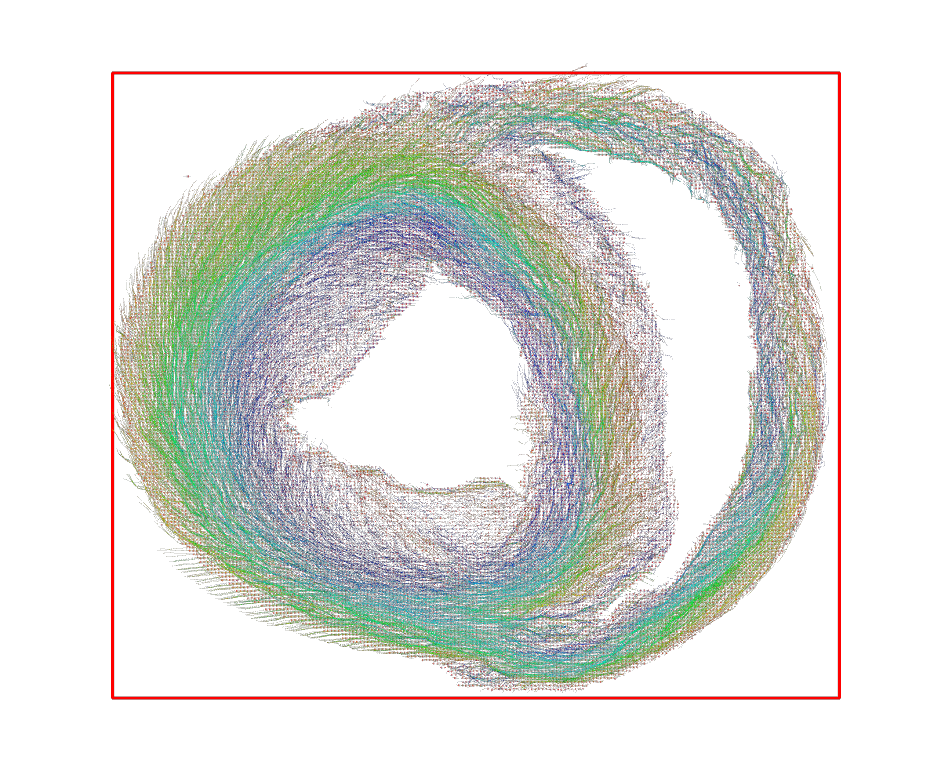
\includegraphics[width=\textwidth]{figures/pig4_topview_tracto_no_smooth}
        \caption{Without any smoothing}
        \label{fig:pig4_tracto_no_smooth}
    \end{subfigure}
    \begin{subfigure}{.48\textwidth}
        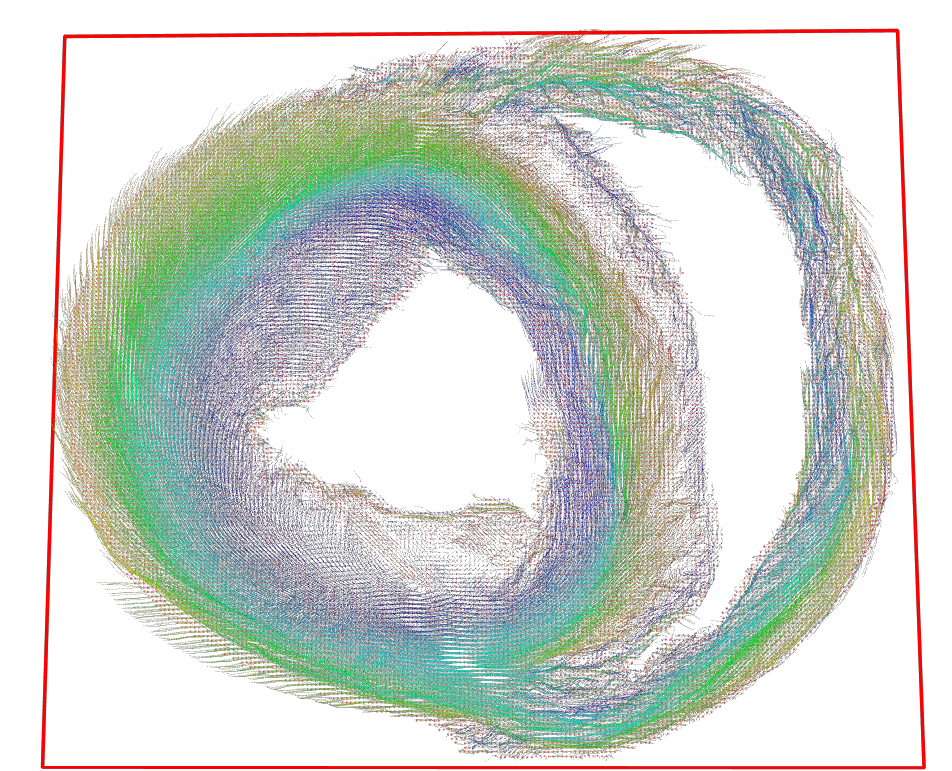
\includegraphics[width=\textwidth]{figures/pig4_topview_tracto_smooth}
        \caption{With Rician smoothing}
        \label{fig:pig4_tracto_smooth}
    \end{subfigure}
    \caption{Tractography of heart fibers for pig 4}
    \label{fig:pig4_tractos}
\end{figure}

\begin{figure}
    \centering
    \begin{subfigure}{.48\textwidth}
        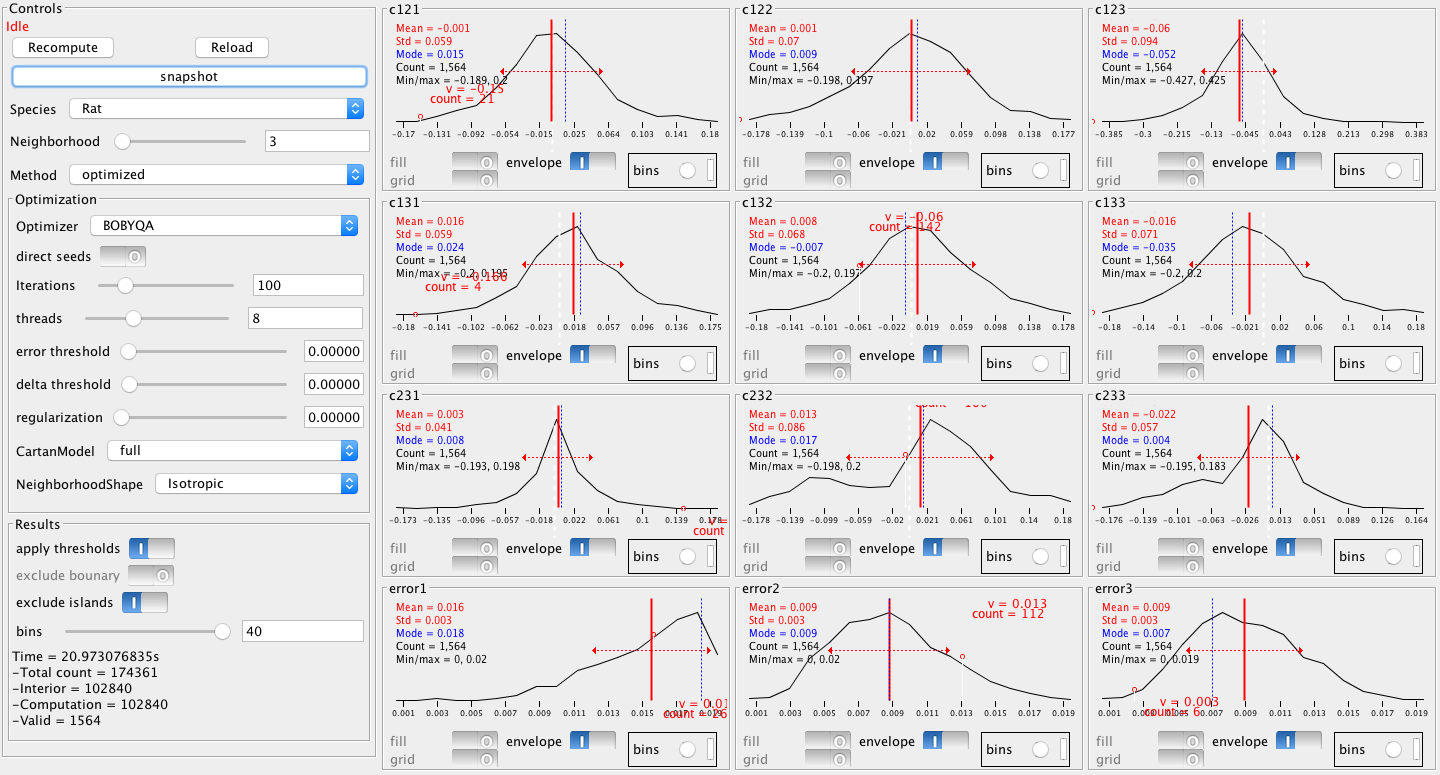
\includegraphics[width=\textwidth]{figures/histogram_pig6_no_smooth}
        \caption{Without any smoothing}
        \label{fig:histogram_pig6_no_smooth}
    \end{subfigure}
    \begin{subfigure}{.48\textwidth}
        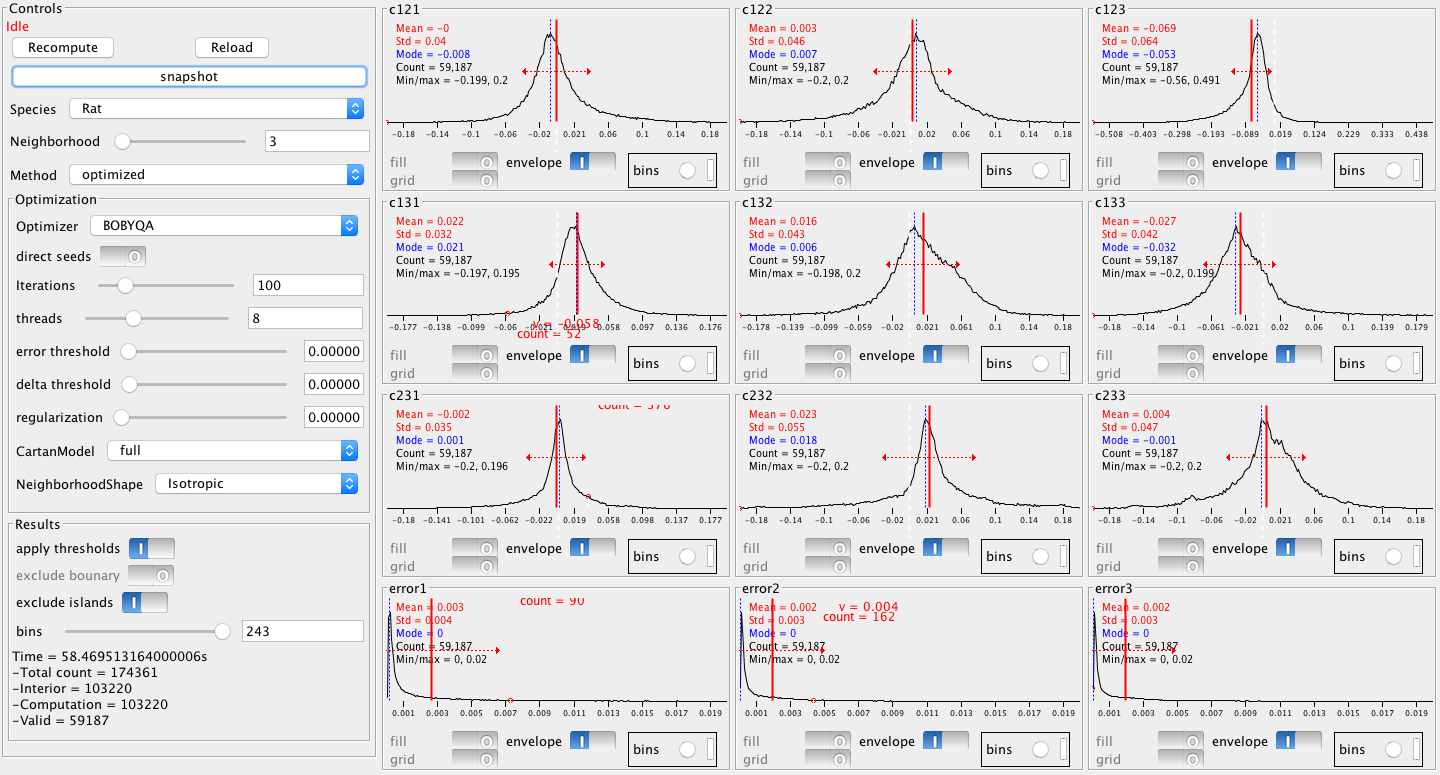
\includegraphics[width=\textwidth]{figures/histogram_pig6_smooth}
        \caption{With Rician smoothing}
        \label{fig:histogram_pig6_smooth}
    \end{subfigure}
    \caption{Histogram of model fitting on raw and smoothed data}
    \label{fig:pig6_histograms}
\end{figure}

\subsection{Error of fit vs ADC and FA}

\begin{figure}
    \centering
    \begin{subfigure}{.31\textwidth}
        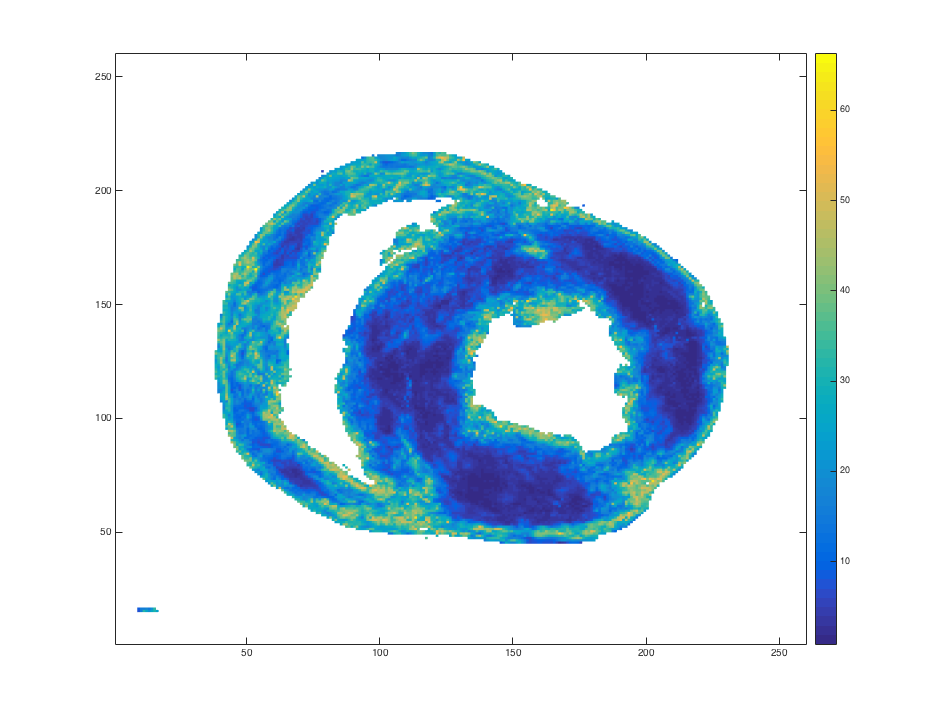
\includegraphics[width=\textwidth]{figures/pig2_err_31}
        \caption{Error of fit}
        \label{fig:pig2_err}
    \end{subfigure}
    \begin{subfigure}{.31\textwidth}
        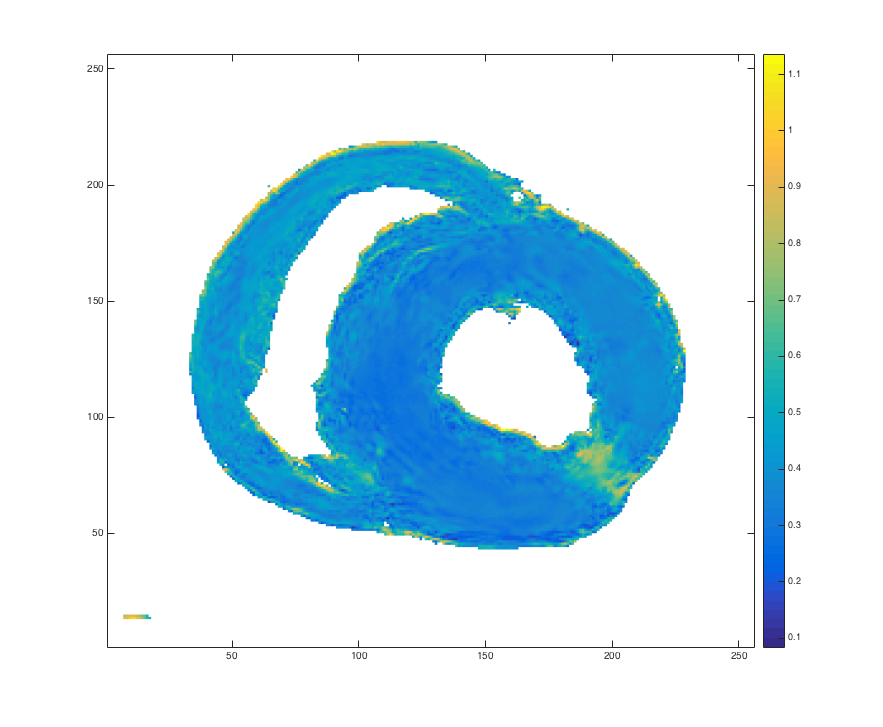
\includegraphics[width=\textwidth]{figures/pig2_adc_31}
        \caption{ADC map}
        \label{fig:pig2_adc}
    \end{subfigure}
    \begin{subfigure}{.31\textwidth}
        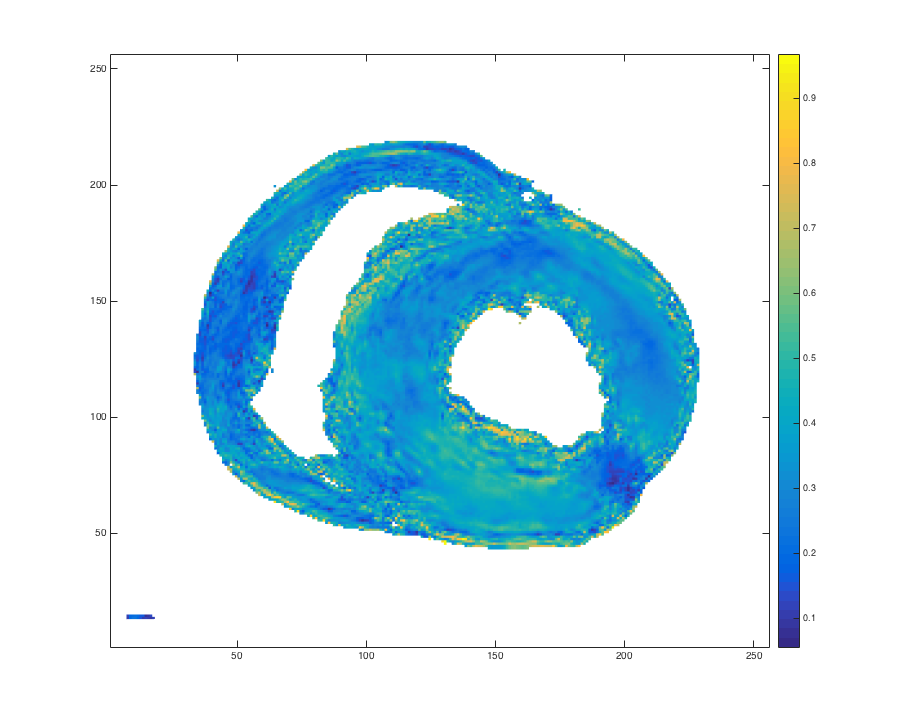
\includegraphics[width=\textwidth]{figures/pig2_fa_31}
        \caption{FA map}
        \label{fig:pig2_fa}
    \end{subfigure}
    \caption{Pig 2: Error of fit computed using our framework compared to ADC and FA map}
    \label{fig:pig2}
\end{figure}

\begin{figure}
    \centering
    \begin{subfigure}{.31\textwidth}
        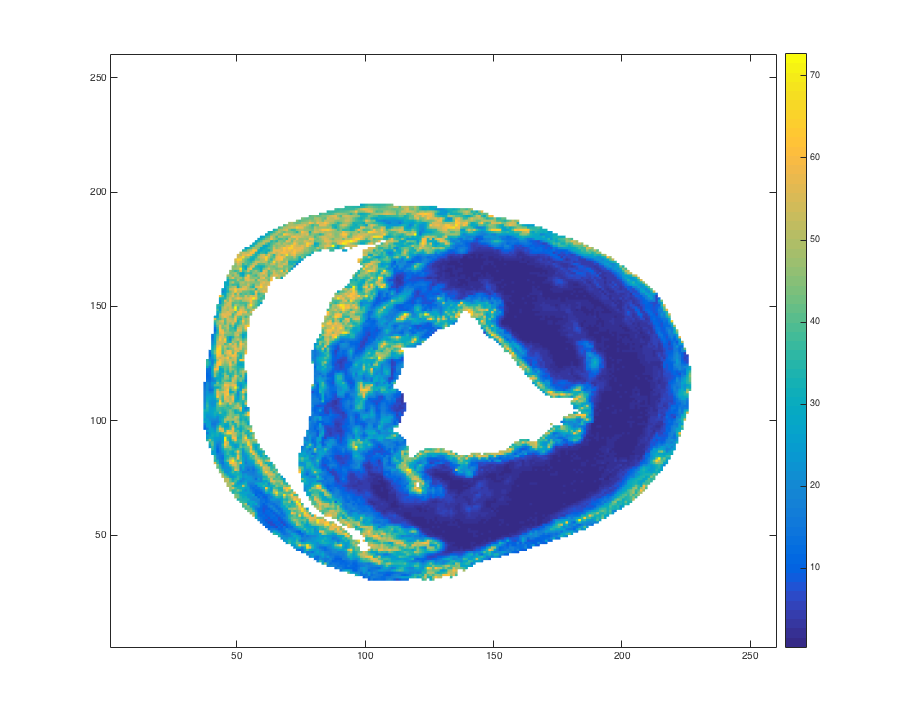
\includegraphics[width=\textwidth]{figures/pig4_err_21}
        \caption{Error of fit}
        \label{fig:pig4_err}
    \end{subfigure}
    \begin{subfigure}{.31\textwidth}
        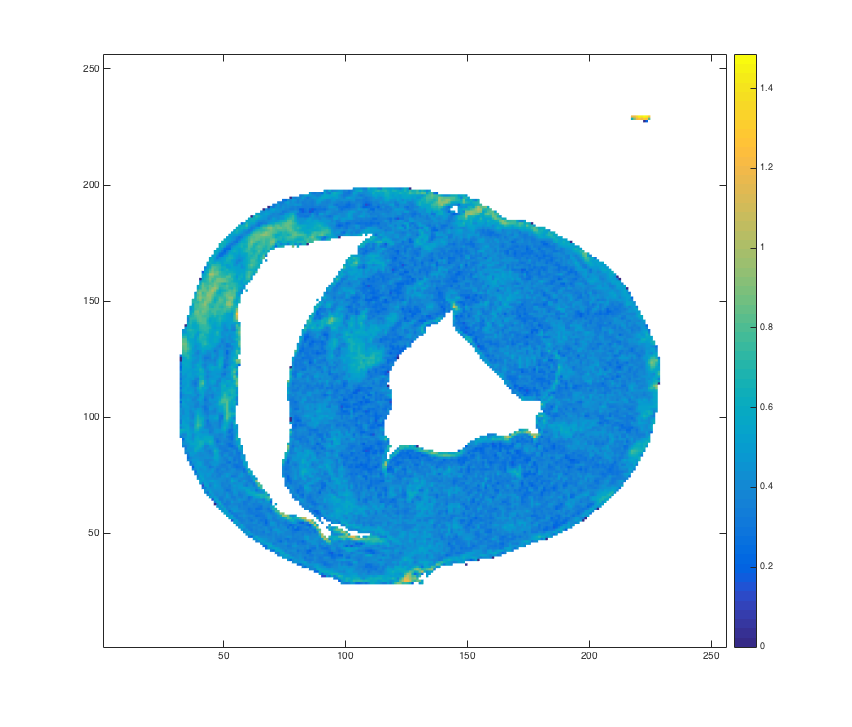
\includegraphics[width=\textwidth]{figures/pig4_adc_21}
        \caption{ADC map}
        \label{fig:pig4_adc}
    \end{subfigure}
    \begin{subfigure}{.31\textwidth}
        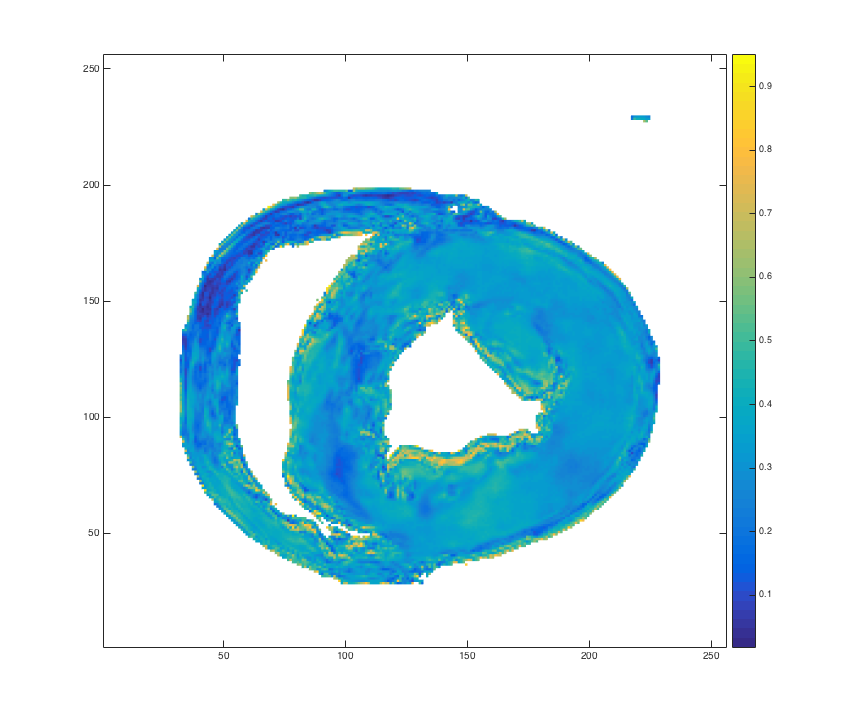
\includegraphics[width=\textwidth]{figures/pig4_fa_21}
        \caption{FA map}
        \label{fig:pig4_fa}
    \end{subfigure}
    \caption{Pig 4: Error of fit computed using our framework compared to ADC and FA map}
    \label{fig:pig4}
\end{figure}

\begin{figure}
    \centering
    \begin{subfigure}{.31\textwidth}
        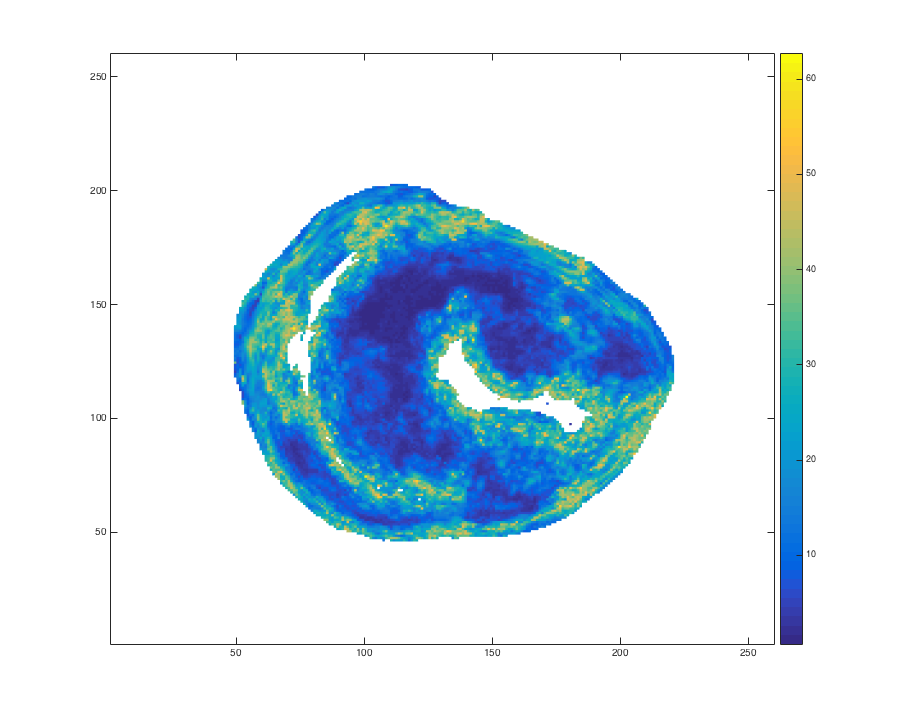
\includegraphics[width=\textwidth]{figures/pig5_err_22}
        \caption{Error of fit}
        \label{fig:pig5_err}
    \end{subfigure}
    \begin{subfigure}{.31\textwidth}
        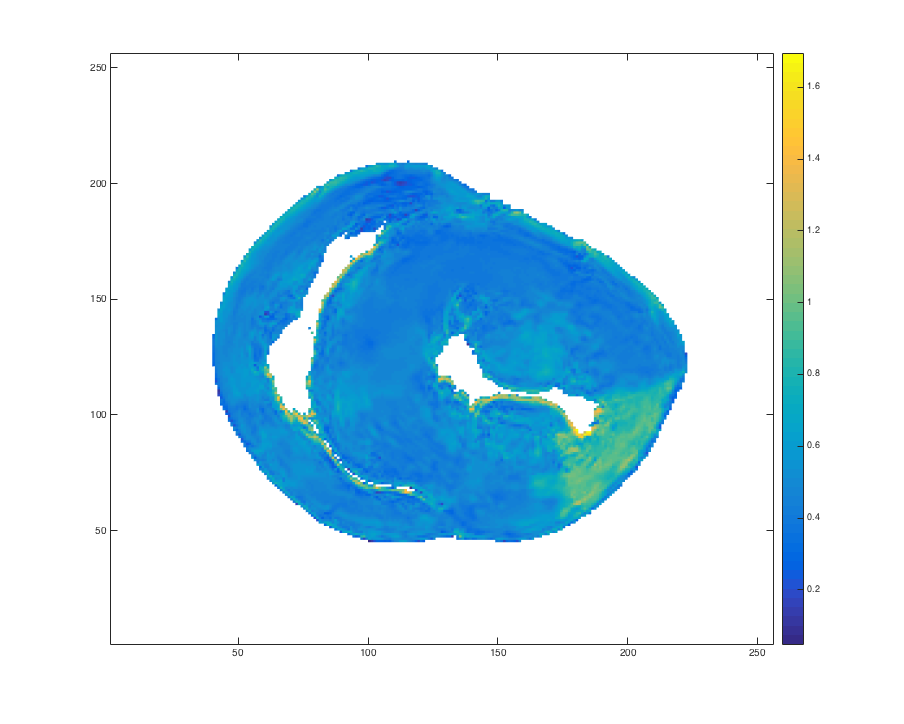
\includegraphics[width=\textwidth]{figures/pig5_adc_22}
        \caption{ADC map}
        \label{fig:pig5_adc}
    \end{subfigure}
    \begin{subfigure}{.31\textwidth}
        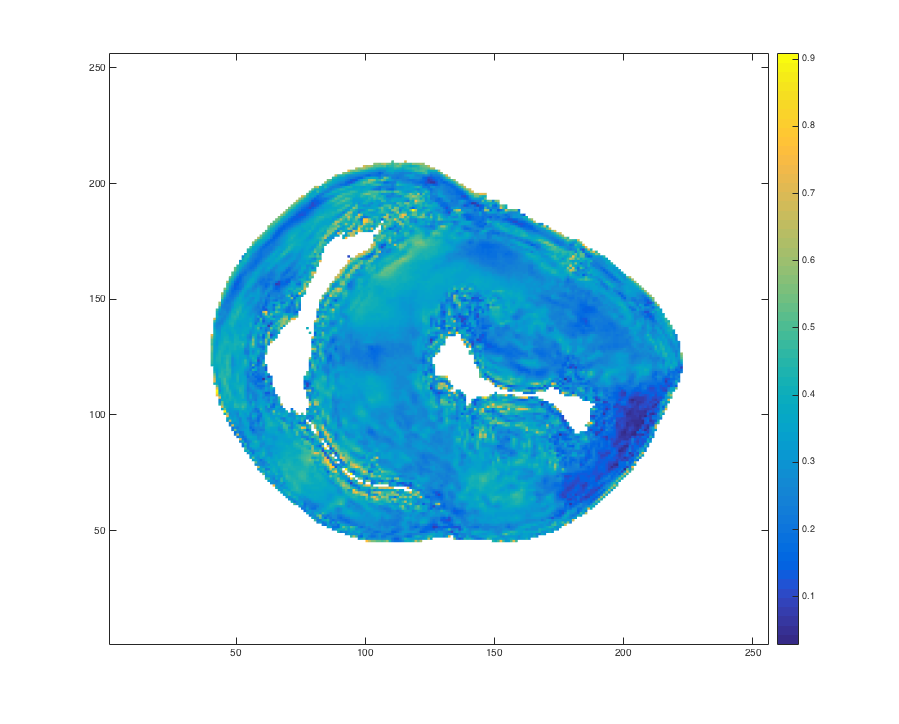
\includegraphics[width=\textwidth]{figures/pig5_fa_22}
        \caption{FA map}
        \label{fig:pig5_fa}
    \end{subfigure}
    \caption{Pig 5: Error of fit computed using our framework compared to ADC and FA map}
    \label{fig:pig5}
\end{figure}

\begin{figure}
    \centering
    \begin{subfigure}{.31\textwidth}
        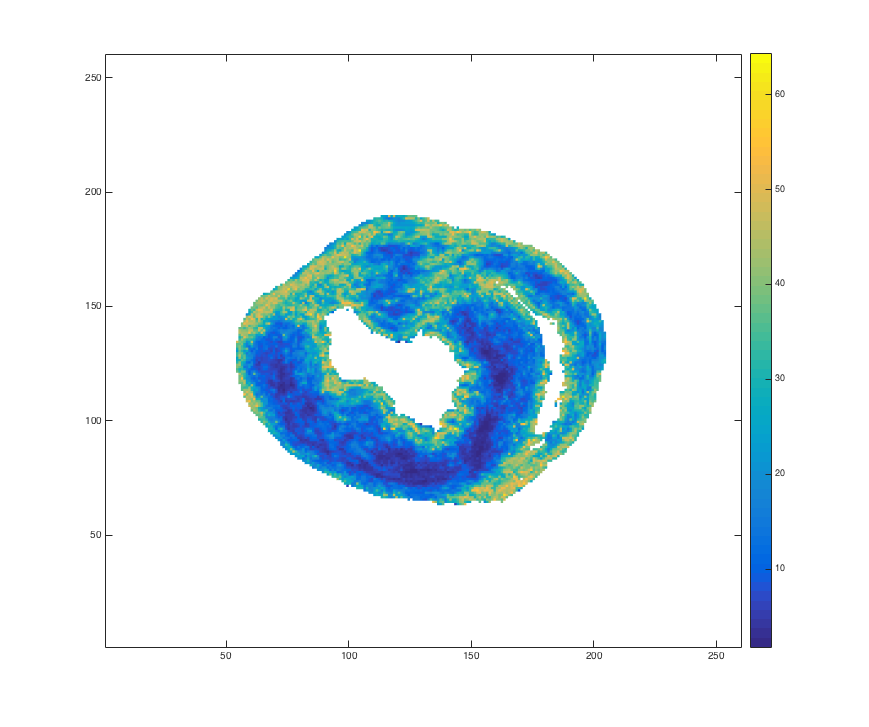
\includegraphics[width=\textwidth]{figures/pig6_err_24}
        \caption{Error of fit}
        \label{fig:pig6_err}
    \end{subfigure}
    \begin{subfigure}{.31\textwidth}
        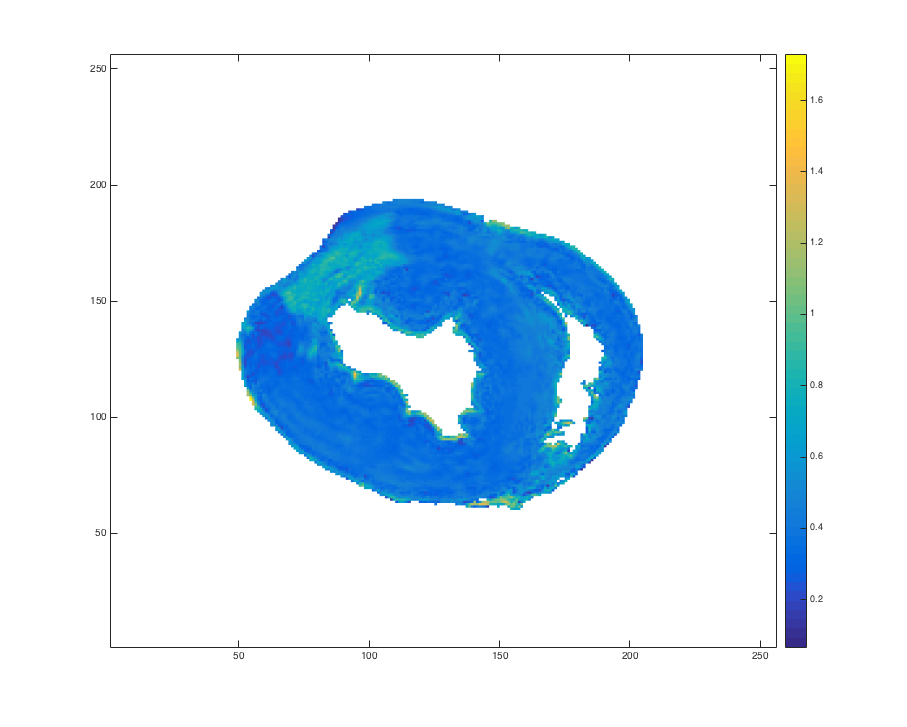
\includegraphics[width=\textwidth]{figures/pig6_adc_24}
        \caption{ADC map}
        \label{fig:pig6_adc}
    \end{subfigure}
    \begin{subfigure}{.31\textwidth}
        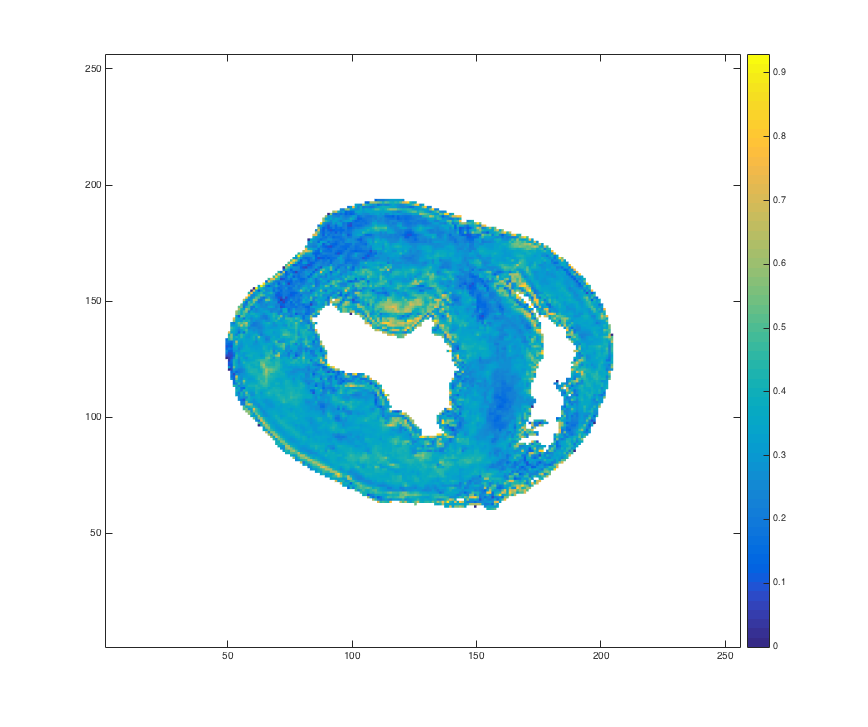
\includegraphics[width=\textwidth]{figures/pig6_fa_24}
        \caption{FA map}
        \label{fig:pig6_fa}
    \end{subfigure}
    \caption{Pig 6: Error of fit computed using our framework compared to ADC and FA map}
    \label{fig:pig6}
\end{figure}

\subsection{Discussion}

Supplementing the earlier results in Fig. 1, Fig 3 compares ADC maps (top row) with our Cartan frame fitting-based error of fit maps in degrees (second row) for a healthy pig heart (left column) and 2 additional infarcted hearts (middle and right columns). In all these examples locations where the ADC value is high are typically also ones where the error of fit is high, with regions of low error of fit being restricted to healthy tissue. In addition though, the error of fit is also consistently high at locations close to the epithelial and endothelial boundaries, signaling a loss in geometric coherence of fibers there. Curiously this phenomena is also seen at the borders of the healthy heart (Fig. 3 left column).

\section{Quantitative Results}

Given the association between ADC and our error of frame fit, it is natural to compare these measures quantitatively throughout the myocardium. We did so for the 5 infarcted porcine hearts we analyzed by computing Dice coefficients to describe the overlap, in the following manner. For the same heart let A be the set of voxels with ADC value > 0.6 and let B be the set of voxels with error of fit > 15 degrees. We computed the standard Dice coefficient A∩B/A∪B as well as a modified coefficient A∩B/A. These results, shown in Table. 1 (left), demonstrate that typically over 80\% of the locations with increased diffusion also yield a high error of fit using our frame fitting method, due to the loss of geometric coherence of fiber orientations. However there are additional locations where fiber orientations are not smooth, typically at the linings of the heart wall, or near the edges of a collapsing and narrow right ventricle. These % Experiment 2

%\chapter{Conclusion}

The study of infarcted pig hearts 6 weeks after infarction has allowed us to compare the more mainstream analytical approach that is ADC and FA maps to our error of fit analysis.

We have noticed difference in the results shown by the more scalar approaches that are ADC and FA compared to our geometrical approach that tries to understand and explain how the tissue is organized and how fibers are oriented if they still exist. As the literature points out, after infarct surviving fiber bundles can persist in the infarct region and have a role in the contraction of the damaged heart. These geometrical reorganization is interesting to observe as it is the cause to tachycardia.

Our error of fit shows efficiently regions of surviving fibers as well as regions with a high concentration of collagen. A more complete study could be interesting if we had access to infarcted hearts at different stages after infarct to see how the reorganization takes place, and if good quality in-vivo MRI images could be obtained then a much better understanding of the effect of the infarct and the cause of tachycardia could be achieved. % Results and Discussion

%\input{Chapters/Chapter7} % Conclusion

%% ----------------------------------------------------------------
% Now begin the Appendices, including them as separate files

\addtocontents{toc}{\vspace{2em}} % Add a gap in the Contents, for aesthetics

\appendix % Cue to tell LaTeX that the following 'chapters' are Appendices

\chapter{An Appendix}
	% Appendix Title

%\input{Appendices/AppendixB} % Appendix Title

%\input{Appendices/AppendixC} % Appendix Title

\addtocontents{toc}{\vspace{2em}}  % Add a gap in the Contents, for aesthetics
\backmatter

%% ----------------------------------------------------------------
\label{Bibliography}
\lhead{\emph{Bibliography}}  % Change the left side page header to "Bibliography"
\bibliographystyle{unsrtnat}  % Use the "unsrtnat" BibTeX style for formatting the Bibliography
\bibliography{Bibliography}  % The references (bibliography) information are stored in the file named "Bibliography.bib"

\end{document}  % The End
%% ----------------------------------------------------------------